%%%%%%%%%%%%%%%%%%%%%%%%%%%%%%%%%%%%%%%%%%%%%%%%%%%%%%%%%%%%%%%%%%%%%%
\section{\label{sec:Configuring-Policy}
Configuring The Startd Policy}
%%%%%%%%%%%%%%%%%%%%%%%%%%%%%%%%%%%%%%%%%%%%%%%%%%%%%%%%%%%%%%%%%%%%%%

\index{configuration!startd policy}
\index{startd!configuration}
\index{daemon!\Condor{startd}}
This section describes the configuration of the \Condor{startd} to
implement the desired policy for when remote jobs should start, be
suspended, (possibly) resumed, vacate (with a checkpoint) or be killed
(no checkpoint).
This policy is the heart of Condor's balancing act
between the needs and wishes of resource owners (machine owners) and
resource users (people submitting their jobs to Condor).
Please read
this section carefully if you plan to change any of the settings
described here, as getting it wrong can have a severe impact on
either the owners of machines in your pool (they may
ask to be removed from the pool entirely) or the users of your pool
(they may stop using Condor).

Before we get into the details, there are a few things to note:
\begin{itemize}
\item Much of this section refers to ClassAd expressions.  You
probably want to read through section~\ref{classad-reference} on
ClassAd expressions before continuing with this.

\item If you are familiar with the version 6.0 policy expressions and
what they do, you read
section~\ref{sec:V60-Policy-diffs} on
page~\pageref{sec:V60-Policy-diffs} which explains the differences
between the version 6.0 policy expressions and later versions.  

\item If you are defining the policy for an SMP (multi-CPU) machine,
also read section~\ref{sec:Configuring-SMP} on
Configuring The Startd for SMP Machines.  
Each \Term{virtual machine} represented by the \condor{startd} on an
SMP machine will have its own \Term{state} and \Term{activity}
(described below). 
In the future, each virtual machine will be able to have its
own policy expressions defined.
For the rest of this section, the word ``machine''
means an individual virtual machine, for
an SMP machine that is showing up as multiple virtual
machines in your pool.  
\end{itemize}

To define your policy, you set expressions in
the configuration file (see section~\ref{sec:Configuring-Condor} on
Configuring Condor for an introduction to Condor's
configuration files).
The expressions are evaluated in the context of the machine's ClassAd
and a job ClassAd.
The expressions can therefore reference attributes from either
ClassAd. 
Listed in this section are
the attributes that are included in the machine's ClassAd and
the attributes that are included in a job ClassAd. 
\index{START@\Expr{START} expression}
\index{configuration!START@\Expr{START} expression}
The \Expr{START} expression, which describes
to Condor what conditions must be met for a machine to start a job
are explained.
The \Expr{RANK} expression is described.
It allows the specification of
the kinds of jobs a machine prefers to run.
A final discussion details how the \Condor{startd} works.
Included are
the machine \Term{states} and \Term{activities}, to give
an idea of what is possible in policy decisions.
Two example policy settings are presented.

%%%%%%%%%%%%%%%%%%%%%%%%%%%%%%%%%%%%%%%%%%%%%%%%%%%%%%%%%%%%%%%%%%%%%%
\subsection{\label{sec:Startd-Attributes}
Startd ClassAd Attributes}
%%%%%%%%%%%%%%%%%%%%%%%%%%%%%%%%%%%%%%%%%%%%%%%%%%%%%%%%%%%%%%%%%%%%%%

\index{\condor{startd}}
The \Condor{startd} represents the machine on which it is running to
the Condor pool.  It publishes characteristics about the
machine in its ClassAd to aid matchmaking with resource requests.
The values of these attributes can be found by using
\Prog{\condor{status} -l hostname}.
On an SMP machine, the startd will break the machine up and advertise
it as separate virtual machines, each with its own name and ClassAd.
The attributes themselves and what they represent are described below:

\begin{description}
%
\index{ClassAd!machine attributes}
\index{ClassAd machine attribute!Activity}
\item[\AdAttr{Activity}:] String which describes HTCondor job activity on the machine.
Can have one of the following values:
	\begin{description}
	\item[\AdStr{Idle}:] There is no job activity
	\item[\AdStr{Busy}:] A job is busy running
	\item[\AdStr{Suspended}:] A job is currently suspended
	\item[\AdStr{Vacating}:] A job is currently checkpointing
	\item[\AdStr{Killing}:] A job is currently being killed
	\item[\AdStr{Benchmarking}:] The startd is running benchmarks
	\item[\AdStr{Retiring}:] Waiting for a job to finish or for the maximum retirement time to expire
	\end{description}
%
\index{ClassAd machine attribute!Arch}
\label{Arch-machine-attribute}
\item[\AdAttr{Arch}:] String with the architecture of the machine.  
Currently supported architectures have the following string
definitions:
	\begin{description}
	\item[\AdStr{INTEL}:] Intel x86 CPU (Pentium, Xeon, etc).
	\item[\AdStr{X86\_64}:] AMD/Intel 64-bit X86
	\end{description}
These strings show definitions for architectures no longer supported:
	\begin{description}
	\item[\AdStr{IA64}:] Intel Itanium
	\item[\AdStr{SUN4u}:] Sun UltraSparc CPU
	\item[\AdStr{SUN4x}:] A Sun Sparc CPU other than an UltraSparc, i.e.
sun4m or sun4c CPU found in older Sparc workstations such as the Sparc~10, 
Sparc~20, IPC, IPX, etc.
	\item[\AdStr{PPC}:] 32-bit PowerPC
	\item[\AdStr{PPC64}:] 64-bit PowerPC
	\end{description}
%
\index{ClassAd machine attribute!CanHibernate}
\item[\AdAttr{CanHibernate}:] The \Condor{startd} has the capability to 
shut down or hibernate a machine when certain configurable criteria are met.
However, before the \Condor{startd} can shut down a machine, 
the hardware itself must support hibernation, as must the operating system. 
When the \Condor{startd} initializes, 
it checks for this support.
If the machine has the ability to hibernate, 
then this boolean ClassAd attribute will be \Expr{True}.
By default, it is \Expr{False}.
%
\index{ClassAd machine attribute!CheckpointPlatform}
\label{CheckpointPlatform-machine-attribute}
\item[\AdAttr{CheckpointPlatform}:] A string which opaquely encodes various
aspects about a machine's operating system, hardware, and kernel
attributes.
It is used to identify systems where previously taken checkpoints for
the standard universe may resume.
%
\index{ClassAd machine attribute!ClockDay}
\item[\AdAttr{ClockDay}:] The day of the week, 
where 0 = Sunday, 1 = Monday, \Dots, and 6 = Saturday. 
%
\index{ClassAd machine attribute!ClockMin}
\item[\AdAttr{ClockMin}:] The number of minutes passed since midnight.
%
\index{ClassAd machine attribute!CondorLoadAvg}
\item[\AdAttr{CondorLoadAvg}:] The load average contributed  
by HTCondor, either from remote jobs or running benchmarks.
%
\index{ClassAd machine attribute!CondorVersion}
\item[\AdAttr{CondorVersion}:] A string containing the HTCondor version
number for the \Condor{startd} daemon, the release date, and the build
identification number.
%
\index{ClassAd machine attribute!ConsoleIdle}
\item[\AdAttr{ConsoleIdle}:] The number of seconds since activity on the system
console keyboard or console mouse has last been detected.
The value can be modified with \Macro{SLOTS\_CONNECTED\_TO\_CONSOLE}
as defined at ~\ref{param:SlotsConnectedToConsole}.
%
\index{ClassAd machine attribute!Cpus}
\item[\AdAttr{Cpus}:]  The number of CPUs in this slot.
It is 1 for a single CPU slot, 2 for a dual CPU slot, etc.
%
\index{ClassAd machine attribute!CurrentRank}
\item[\AdAttr{CurrentRank}:] A float which represents this machine
owner's affinity
for running the HTCondor job which it is currently hosting.  If not
currently hosting an HTCondor job, \AdAttr{CurrentRank} is 0.0.
When a machine is claimed,
the attribute's value is computed by evaluating the machine's
\AdAttr{Rank} expression with respect to the current job's ClassAd.
%
\index{ClassAd machine attribute!Disk}
\item[\AdAttr{Disk}:] The amount of disk space on this machine available for
the job in Kbytes ( e.g. 23000 = 23 megabytes ).  Specifically, this
is the amount of disk space available in the directory specified in
the HTCondor configuration files by the \Macro{EXECUTE} macro, minus any
space reserved with the \Macro{RESERVED\_DISK} macro.
%
\index{ClassAd machine attribute!Draining}
\item[\AdAttr{Draining}:] This attribute is \Expr{True} when the slot
is draining and undefined if not.
%
\index{ClassAd machine attribute!DrainingRequestId}
\item[\AdAttr{DrainingRequestId}:] This attribute contains a string that
is the request id of the draining request that put this slot in a draining
state.  It is undefined if the slot is not draining.
%
\index{ClassAd machine attribute!DotNetVersions}
\item[\AdAttr{DotNetVersions}:] The .NET framework versions
currently installed on this computer. 
Default format is a comma delimited list. 
Current definitions:
  \begin{description}
  \item[\AdStr{1.1}:] for .Net Framework 1.1
  \item[\AdStr{2.0}:] for .Net Framework 2.0
  \item[\AdStr{3.0}:] for .Net Framework 3.0
  \item[\AdStr{3.5}:] for .Net Framework 3.5
  \item[\AdStr{4.0Client}:] for .Net Framework 4.0 Client install
  \item[\AdStr{4.0Full}:] for .Net Framework 4.0 Full install
  \end{description}
%
\index{ClassAd machine attribute!DynamicSlot}
\label{DynamicSlot-machine-attribute} 
\item[\AdAttr{DynamicSlot}:] For SMP machines that allow dynamic
partitioning of a slot,
this boolean value identifies that this dynamic slot may be partitioned.
%
\index{ClassAd machine attribute!EnteredCurrentActivity}
\item[\AdAttr{EnteredCurrentActivity}:] Time at which the machine
entered the current Activity (see \AdAttr{Activity} entry above).  On
all platforms (including NT), this is measured in the number of
integer seconds since the Unix epoch (00:00:00 UTC, Jan 1, 1970).
%
\index{ClassAd machine attribute!ExpectedMachineGracefulDrainingBadput}
\item[\AdAttr{ExpectedMachineGracefulDrainingBadput}:] The
job runtime in cpu-seconds that would be lost if graceful draining
were initiated at the time this ad was published.  This calculation assumes
that jobs will run for the full retirement time and then be evicted
without saving a checkpoint.
%
\index{ClassAd machine attribute!ExpectedMachineGracefulDrainingCompletion}
\item[\AdAttr{ExpectedMachineGracefulDrainingCompletion}:] Time at
which graceful draining of the machine could complete if it were
initiated at the time this ad was published.  This is measured in the
number of integer seconds since the Unix epoch (00:00:00 UTC, Jan 1,
1970).  This value is computed with the assumption that the machine
policy will not suspend jobs during draining while the machine is
waiting for the job to use up its retirement time.  If suspension
happens, the upper bound on how long draining could take is
unlimited.  To avoid suspension during draining, the \MacroNI{SUSPEND}
and \MacroNI{CONTINUE} expressions could be configured to pay
attention to the \AdAttr{Draining} attribute.
%
\index{ClassAd machine attribute!ExpectedMachineQuickDrainingBadput}
\item[\AdAttr{ExpectedMachineGracefulQuickBadput}:] The
job runtime in cpu-seconds that would be lost if quick draining
were initiated at the time this ad was published.  This calculation assumes
that all evicted jobs will not save a checkpoint.
%
\index{ClassAd machine attribute!ExpectedMachineQuickDrainingCompletion}
\item[\AdAttr{ExpectedMachineQuickDrainingCompletion}:] Time at
which quick draining of the machine could complete if it were
initiated at the time this ad was published.  This is measured in the
number of integer seconds since the Unix epoch (00:00:00 UTC, Jan 1,
1970).
%
\index{ClassAd machine attribute!FileSystemDomain}
\item[\AdAttr{FileSystemDomain}:] A domain name configured by the
HTCondor administrator which describes a cluster of machines which all
access the same, uniformly-mounted, networked file systems usually via
NFS or AFS.  This is useful for Vanilla universe jobs which require
remote file access.
%
\index{ClassAd machine attribute!Has\_sse4\_1}
\item[\AdAttr{Has\_sse4\_1}:] A boolean value set to \Expr{True}
 if the machine being advertised supports
the SSE 4.1 instructions, and \Expr{Undefined} otherwise.
%
\index{ClassAd machine attribute!Has\_sse4\_2}
\item[\AdAttr{Has\_sse4\_2}:] A boolean value set to \Expr{True}
if the machine being advertised supports
the SSE 4.2 instructions, and \Expr{Undefined} otherwise.
%
\index{ClassAd machine attribute!has\_ssse3}
\item[\AdAttr{has\_ssse3}:] A boolean value set to \Expr{True}
if the machine being advertised supports
the SSSE 3 instructions, and \Expr{Undefined} otherwise.
%
\index{ClassAd machine attribute!HasVM}
\item[\AdAttr{HasVM}:] A boolean value added to the machine ClassAd
when the configuration triggers the detection of virtual machine
software.
%
\index{ClassAd machine attribute!IsWakeAble}
\item[\AdAttr{IsWakeAble}:] A boolean value that when \Expr{True} identifies
that the machine has the capability to be woken into a 
fully powered and running state by receiving a Wake On LAN (WOL) packet.
This ability is a function of the operating system, 
the network adapter in the machine 
(notably, wireless network adapters usually do not have this function),
and BIOS settings. 
When the \Condor{startd} initializes, 
it tries to detect if the operating system and network adapter both support 
waking from hibernation by receipt of a WOL packet.
The default value is \Expr{False}.
%
\index{ClassAd machine attribute!IsWakeEnabled}
\item[\AdAttr{IsWakeEnabled}:] If the hardware and software have the capacity 
to be woken into a fully powered and running state by receiving 
a Wake On LAN (WOL) packet,
this feature can still be disabled via the BIOS or software.
If BIOS or the operating system have disabled this feature, 
the \Condor{startd} sets this boolean attribute to \Expr{False}.
%
\index{ClassAd machine attribute!JobVM\_VCPUS}
\item[\AdAttr{JobVM\_VCPUS}:] An attribute defined if a vm universe job
is running on this slot.  Defined by the number of virtualized CPUs
in the virtual machine.
%
\index{ClassAd machine attribute!KeyboardIdle}
\item[\AdAttr{KeyboardIdle}:] The number of seconds since activity on any
keyboard or mouse associated with this machine has last been detected.
Unlike \AdAttr{ConsoleIdle}, \AdAttr{KeyboardIdle} also takes activity 
on pseudo-terminals into
account.
Pseudo-terminals have virtual keyboard activity from telnet and rlogin
sessions.  Note that \AdAttr{KeyboardIdle} will always be equal to or
less than \AdAttr{ConsoleIdle}.
The value can be modified with \Macro{SLOTS\_CONNECTED\_TO\_KEYBOARD}
as defined at ~\ref{param:SlotsConnectedToKeyboard}.
%
\index{ClassAd machine attribute!KFlops}
\item[\AdAttr{KFlops}:] Relative floating point performance as determined via a
Linpack benchmark.
%
\index{ClassAd machine attribute!LastDrainStartTime}
\item[\AdAttr{LastDrainStartTime}:] Time when draining of this
\Condor{startd} was last initiated (e.g. due to \Condor{defrag} or
\Condor{drain}).
%
\index{ClassAd machine attribute!LastHeardFrom}
\item[\AdAttr{LastHeardFrom}:] Time when the HTCondor central manager last
received a status update from this machine.  
Expressed as 
the number of integer seconds since the Unix epoch (00:00:00 UTC, Jan 1, 1970).
Note: This attribute is only inserted by the central manager once it
receives the ClassAd.
It is not present in the \Condor{startd} copy of the ClassAd.
Therefore, you could not use this attribute in defining \Condor{startd}
expressions (and you would not want to).
%
\index{ClassAd machine attribute!LoadAvg}
\item[\AdAttr{LoadAvg}:] A floating point number representing the 
current load average.
%
\index{ClassAd machine attribute!Machine}
\item[\AdAttr{Machine}:] A string with the machine's fully qualified host name.
%
\index{ClassAd machine attribute!MachineMaxVacateTime}
\item[\AdAttr{MachineMaxVacateTime}:] An integer expression that specifies
the time in seconds the machine will allow the job to gracefully shut
down.
%
\index{ClassAd machine attribute!Memory}
\item[\AdAttr{Memory}:] The amount of RAM in megabytes.
%
\index{ClassAd machine attribute!Mips}
\item[\AdAttr{Mips}:] Relative integer performance as determined via a Dhrystone
benchmark.

\index{ClassAd machine attribute!MonitorSelfAge}
\item[\AdAttr{MonitorSelfAge}:] The number of seconds that this daemon
  has been running.

\index{ClassAd machine attribute!MonitorSelfCPUUsage}
\item[\AdAttr{MonitorSelfCPUUsage}:] The fraction of recent CPU time utilized
  by this daemon. 

\index{ClassAd machine attribute!MonitorSelfImageSize}
\item[\AdAttr{MonitorSelfImageSize}:] The amount of virtual memory consumed by
  this daemon in Kbytes.

\index{ClassAd machine attribute!MonitorSelfRegisteredSocketCount}
\item[\AdAttr{MonitorSelfRegisteredSocketCount}:] The current number of sockets
  registered by this daemon.

\index{ClassAd machine attribute!MonitorSelfResidentSetSize}
\item[\AdAttr{MonitorSelfResidentSetSize}:] The amount of resident memory
  used by this daemon in Kbytes.

\index{ClassAd machine attribute!MonitorSelfSecuritySessions}
\item[\AdAttr{MonitorSelfSecuritySessions}:] The number of open (cached)
  security sessions for this daemon.

\index{ClassAd machine attribute!MonitorSelfTime}
\item[\AdAttr{MonitorSelfTime}:] The  time, represented as the number of
  second elapsed since the Unix epoch (00:00:00 UTC, Jan 1, 1970),
  at which this daemon last checked and set the attributes with names that
  begin with the string \Attr{MonitorSelf}.
  
\index{ClassAd machine attribute!MyAddress}
\item[\AdAttr{MyAddress}:] String with the IP and port address of the
\Condor{startd} daemon which is publishing this machine ClassAd.
When using CCB, \Condor{shared\_port}, and/or an additional private
network interface, that information will be included here as well.

\index{ClassAd machine attribute!MyType}
\item[\AdAttr{MyType}:] The ClassAd type; always set to the literal string \AdStr{Machine}.
%
\index{ClassAd machine attribute!Name}
\item[\AdAttr{Name}:] The name of this resource; typically the same value as
the \AdAttr{Machine} attribute, but could be customized by the site
administrator.
On SMP machines, the \Condor{startd} will divide the CPUs up into separate
slots, each with with a unique name.
These names will be of the form ``slot\#@full.hostname'', for example,
``slot1@vulture.cs.wisc.edu'', which signifies slot number 1 from
vulture.cs.wisc.edu.
%
\index{ClassAd machine attribute!OpSys}
\label{OpSys-machine-attribute}
\item[\AdAttr{OpSys}:] String describing the operating system running on this
machine.  
Currently supported operating systems have the following string
definitions:
	\begin{description}
	\item[\AdStr{LINUX}:] for LINUX 2.0.x, LINUX 2.2.x,
	LINUX 2.4.x, LINUX 2.6.x, or LINUX 3.10.0 kernel systems, as well as Scientific Linux 
        and Ubuntu 12.04
	\item[\AdStr{OSX}:] for Darwin
	\item[\AdStr{FREEBSD7}:] for FreeBSD 7
	\item[\AdStr{FREEBSD8}:] for FreeBSD 8
	\item[\AdStr{WINDOWS}:] for all versions of Windows
	\item[\AdStr{SOLARIS5.10}:] for Solaris 2.10 or 5.10
	\item[\AdStr{SOLARIS5.11}:] for Solaris 2.11 or 5.11
	\end{description}
These strings show definitions for operating systems no longer supported:
	\begin{description}
	\item[\AdStr{SOLARIS28}:] for Solaris 2.8 or 5.8
	\item[\AdStr{SOLARIS29}:] for Solaris 2.9 or 5.9
	\end{description}
%
\index{ClassAd machine attribute!OpSysAndVer}
\item[\AdAttr{OpSysAndVer}:] A string indicating an operating system and
a version number.

For Linux operating systems, it is the value of the \Attr{OpSysName} attribute 
concatenated with the string version of the \Attr{OpSysMajorVersion} attribute:
	\begin{description}
	\item[\AdStr{RedHat5}:] for RedHat Linux version 5
	\item[\AdStr{RedHat6}:] for RedHat Linux version 6
	\item[\AdStr{RedHat7}:] for RedHat Linux version 7 \emph{Beta}
	\item[\AdStr{Fedora16}:] for Fedora Linux version 16
	\item[\AdStr{Debian5}:] for Debian Linux version 5
	\item[\AdStr{Debian6}:] for Debian Linux version 6
	\item[\AdStr{Ubuntu12}:] for Ubuntu 12.04
	\item[\AdStr{SL5}:] for Scientific Linux version 5
	\item[\AdStr{SL6}:] for Scientific Linux version 6
	\item[\AdStr{SLFermi5}:] for Fermi's Scientific Linux version 5
	\item[\AdStr{SLFermi6}:] for Fermi's Scientific Linux version 6
	\item[\AdStr{SLCern5}:] for CERN's Scientific Linux version 5
	\item[\AdStr{SLCern6}:] for CERN's Scientific Linux version 6
	\end{description}
For MacOS operating systems, it is the value of the \Attr{OpSysShortName} 
attribute concatenated with the string version of the \Attr{OpSysVer} attribute: 
	\begin{description}
	\item[\AdStr{MacOSX605}:] for MacOS version 10.6.5 (Snow Leopard)
	\item[\AdStr{MacOSX703}:] for MacOS version 10.7.3 (Lion)
	\end{description}
For BSD operating systems, it is the value of the \Attr{OpSysName} attribute 
concatenated with the string version of the \Attr{OpSysMajorVersion} attribute:
	\begin{description}
	\item[\AdStr{FREEBSD7}:] for FreeBSD version 7
	\item[\AdStr{FREEBSD8}:] for FreeBSD version 8
	\end{description}
For Solaris Unix operating systems, 
it is the same value as the \Attr{OpSys} attribute: 
	\begin{description}
	\item[\AdStr{SOLARIS5.10}:] for Solaris 2.10 or 5.10
	\item[\AdStr{SOLARIS5.11}:] for Solaris 2.11 or 5.11
	\end{description}
For Windows operating systems, it is the value of the \Attr{OpSys} attribute 
concatenated with the string version of the \Attr{OpSysMajorVersion} attribute:
	\begin{description}
	\item[\AdStr{WINDOWS500}:] for Windows 2000
	\item[\AdStr{WINDOWS501}:] for Windows XP
	\item[\AdStr{WINDOWS502}:] for Windows Server 2003
	\item[\AdStr{WINDOWS600}:] for Windows Vista
	\item[\AdStr{WINDOWS601}:] for Windows 7
	\end{description}
%
\index{ClassAd machine attribute!OpSysLegacy}
\item[\AdAttr{OpSysLegacy}:] A string that holds the long-standing values for the \Attr{OpSys} attribute.
Currently supported operating systems have the following string
definitions:
	\begin{description}
	\item[\AdStr{LINUX}:] for LINUX 2.0.x, LINUX 2.2.x, LINUX 2.4.x, LINUX 2.6.x, or LINUX 3.10.0 kernel systems, as well as Scientific Linux and  Ubuntu 12.04 versions
	\item[\AdStr{OSX}:] for Darwin
	\item[\AdStr{FREEBSD7}:] for FreeBSD version 7
	\item[\AdStr{FREEBSD8}:] for FreeBSD version 8
	\item[\AdStr{SOLARIS5.10}:] for Solaris 2.10 or 5.10
	\item[\AdStr{SOLARIS5.11}:] for Solaris 2.11 or 5.11
	\item[\AdStr{WINDOWS}:] for all versions of Windows
	\end{description}
%
\index{ClassAd machine attribute!OpSysLongName}
\item[\AdAttr{OpSysLongName}:] A string giving a full description of 
the operating system.
For Linux platforms, this is generally the string taken from \File{/etc/hosts},
with extra characters stripped off Debian versions.
	\begin{description}
	\item[\AdStr{Red Hat Enterprise Linux Server release 5.7 (Tikanga)}:] for RedHat Linux version 5
	\item[\AdStr{Red Hat Enterprise Linux Server release 6.2 (Santiago)}:] for RedHat Linux version 6
	\item[\AdStr{Red Hat Enterprise Linux Everything release 7.0 (Maipo)}:] for RedHat Linux version 7.0 \emph{Beta}
	\item[\AdStr{Ubuntu 12.04.3 LTS}:] for Ubuntu 12.04 point release 3 
	\item[\AdStr{Fedora release 16 (Verne)}:] for Fedora Linux version 16
	\item[\AdStr{MacOSX 6.5}:] for MacOS version 10.6.5 (Snow Leopard)
	\item[\AdStr{MacOSX 7.3}:] for MacOS version 10.7.3 (Lion)
	\item[\AdStr{FreeBSD8.2-RELEASE-p3}:] for FreeBSD version 8
	\item[\AdStr{SOLARIS5.10}:] for Solaris 2.10 or 5.10
	\item[\AdStr{SOLARIS5.11}:] for Solaris 2.11 or 5.11
	\item[\AdStr{Windows XP SP3}:] for Windows XP
	\item[\AdStr{Windows 7 SP2}:] for Windows 7
	\end{description}
%
\index{ClassAd machine attribute!OpSysMajorVersion}
\item[\AdAttr{OpSysMajorVersion}:] An integer value representing the major version of the operating system.
	\begin{description}
	\item[\Expr{5}:] for RedHat Linux version 5 
and derived platforms such as Scientific Linux
	\item[\Expr{6}:] for RedHat Linux version 6
and derived platforms such as Scientific Linux
	\item[\Expr{7}:] for RedHat Linux version 7 \emph{Beta}
	\item[\Expr{12}:] for Ubuntu 12.04
	\item[\Expr{16}:] for Fedora Linux version 16
	\item[\Expr{6}:] for MacOS version 10.6.5 (Snow Leopard)
	\item[\Expr{7}:] for MacOS version 10.7.3 (Lion)
	\item[\Expr{7}:] for FreeBSD version 7
	\item[\Expr{8}:] for FreeBSD version 8
	\item[\Expr{5}:] for Solaris 2.10, 5.10, 2.11, or 5.11
	\item[\Expr{501}:] for Windows XP
	\item[\Expr{600}:] for Windows Vista
	\item[\Expr{601}:] for Windows 7
	\end{description}
%
\index{ClassAd machine attribute!OpSysName}
\item[\AdAttr{OpSysName}:] A string containing a terse description of the operating system.
	\begin{description}
	\item[\AdStr{RedHat}:] for RedHat Linux version 6 and 7 \emph{Beta}
	\item[\AdStr{Fedora}:] for Fedora Linux version 16
	\item[\AdStr{Ubuntu}:] for Ubuntu 12.04
	\item[\AdStr{SnowLeopard}:] for MacOS version 10.6.5 (Snow Leopard)
	\item[\AdStr{Lion}:] for MacOS version 10.7.3 (Lion)
	\item[\AdStr{FREEBSD}:] for FreeBSD version 7 or 8
	\item[\AdStr{SOLARIS5.10}:] for Solaris 2.10 or 5.10
	\item[\AdStr{SOLARIS5.11}:] for Solaris 2.11 or 5.11
	\item[\AdStr{WindowsXP}:] for Windows XP
	\item[\AdStr{WindowsVista}:] for Windows Vista
	\item[\AdStr{Windows7}:] for Windows 7
	\item[\AdStr{SL}:] for Scientific Linux
	\item[\AdStr{SLFermi}:] for Fermi's Scientific Linux
	\item[\AdStr{SLCern}:] for CERN's Scientific Linux
	\end{description}
%
\index{ClassAd machine attribute!OpSysShortName}
\item[\AdAttr{OpSysShortName}:] A string containing a short name for
the operating system.
	\begin{description}
	\item[\AdStr{RedHat}:] for RedHat Linux version 5, 6 or 7 \emph{Beta}
	\item[\AdStr{Fedora}:] for Fedora Linux version 16
	\item[\AdStr{Debian}:] for Debian Linux version 5 or 6
	\item[\AdStr{Ubuntu}:] for Ubuntu 12.04
	\item[\AdStr{MacOSX}:] for MacOS version 10.6.5 (Snow Leopard) or 
for MacOS version 10.7.3 (Lion)
	\item[\AdStr{FreeBSD}:] for FreeBSD version 7 or 8
	\item[\AdStr{SOLARIS5.10}:] for Solaris 2.10 or 5.10
	\item[\AdStr{SOLARIS5.11}:] for Solaris 2.11 or 5.11
	\item[\AdStr{XP}:] for Windows XP
	\item[\AdStr{Vista}:] for Windows Vista
	\item[\AdStr{7}:] for Windows 7
	\item[\AdStr{SL}:] for Scientific Linux
	\item[\AdStr{SLFermi}:] for Fermi's Scientific Linux
	\item[\AdStr{SLCern}:] for CERN's Scientific Linux
	\end{description}
%
\index{ClassAd machine attribute!OpSysVer}
\item[\AdAttr{OpSysVer}:] An integer value representing the operating system
version number.
	\begin{description}
	\item[\Expr{700}:] for RedHat Linux version 7.0 \emph{Beta}
	\item[\Expr{602}:] for RedHat Linux version 6.2
	\item[\Expr{1600}:] for Fedora Linux version 16.0
	\item[\Expr{1204}:] for Ubuntu 12.04
	\item[\Expr{704}:] for FreeBSD version 7.4
	\item[\Expr{802}:] for FreeBSD version 8.2
	\item[\Expr{605}:] for MacOS version 10.6.5 (Snow Leopard)
	\item[\Expr{703}:] for MacOS version 10.7.3 (Lion)
	\item[\Expr{500}:] for Windows 2000
	\item[\Expr{501}:] for Windows XP
	\item[\Expr{502}:] for Windows Server 2003
	\item[\Expr{600}:] for Windows Vista or Windows Server 2008
	\item[\Expr{601}:] for Windows 7 or Windows Server 2008
	\end{description}
%
\index{ClassAd machine attribute!Requirements}
\item[\AdAttr{Requirements}:] A boolean, which when evaluated within the context
of the machine ClassAd and a job ClassAd, must evaluate to
TRUE before HTCondor will allow the job to use this machine.
%
\index{ClassAd machine attribute!MaxJobRetirementTime}
\item[\AdAttr{MaxJobRetirementTime}:] When the \Condor{startd} wants
to kick the job off, a job which has run for less than this number
of seconds will not be hard-killed.  The \Condor{startd} will wait
for the job to finish or to exceed this amount of time, whichever
comes sooner.  If the job vacating policy grants the job X seconds
of vacating time, a preempted job will be soft-killed X seconds
before the end of its retirement time, so that hard-killing of the
job will not happen until the end of the retirement time if the job
does not finish shutting down before then.  This is an expression
evaluated in the context of the job ClassAd, so it may refer to job
attributes as well as machine attributes.
%
\index{ClassAd machine attribute!RetirementTimeRemaining}
\item[\AdAttr{RetirementTimeRemaining}:] An integer number of seconds
after \AdAttr{MyCurrentTime} when the running job can be evicted.
\AdAttr{MaxJobRetirementTime} is the expression of how much retirement
time the machine offers to new jobs, whereas \AdAttr{RetirementTimeRemaining}
is the negotiated amount of time remaining for the current running
job.  This may be less than the amount offered by the machine's
\AdAttr{MaxJobRetirementTime} expression, because the job may
ask for less.
%
\index{ClassAd machine attribute!PartitionableSlot}
\label{PartitionableSlot-machine-attribute} 
\item[\AdAttr{PartitionableSlot}:] For SMP machines,
a boolean value identifying that this slot may be partitioned.
%
\index{ClassAd machine attribute!SlotID}
\item[\AdAttr{SlotID}:] For SMP machines, the integer
that identifies the slot.
The value will be \verb@X@ for the slot with 
\begin{verbatim}
name="slotX@full.hostname"
\end{verbatim}
For non-SMP machines with one slot, the value will be 1.
\Note This attribute was added in HTCondor version 6.9.3.
For older versions of HTCondor, see \AdAttr{VirtualMachineID} below.
%
\index{ClassAd machine attribute!SlotWeight}
\item[\AdAttr{SlotWeight}:]
  This specifies the weight of the slot when
  calculating usage, computing fair shares, and enforcing group
  quotas.  For example, claiming a slot with \Expr{SlotWeight = 2} is
  equivalent to claiming two \Expr{SlotWeight = 1} slots.
  See the description of \MacroNI{SlotWeight} on
  page~\pageref{param:SlotWeight}.

%
\index{ClassAd machine attribute!StartdIpAddr}
\item[\AdAttr{StartdIpAddr}:] String with the IP and port address of the
\Condor{startd} daemon which is publishing this machine ClassAd.
When using CCB, \Condor{shared\_port}, and/or an additional private
network interface, that information will be included here as well.

%
\index{ClassAd machine attribute!State}
\item[\AdAttr{State}:] String which publishes the machine's HTCondor state.
Can be:
	\begin{description}
	\item[\AdStr{Owner}:] The machine owner is using the machine, and
it is unavailable to HTCondor.
	\item[\AdStr{Unclaimed}:] The machine is available to run HTCondor jobs,
but a good match is either not available or not 
yet found.
	\item[\AdStr{Matched}:] The HTCondor central manager has found a good
match for this resource, but an HTCondor scheduler has not yet claimed it.
	\item[\AdStr{Claimed}:] The machine is claimed by a remote
\Condor{schedd} and is probably running a job.
	\item[\AdStr{Preempting}:] An HTCondor job is being preempted (possibly
via checkpointing) in order to clear the machine for either a higher
priority job or because the machine owner wants the machine back.
	\item[\AdStr{Drained}:] This slot is not accepting jobs,
because the machine is being drained.
	\end{description}   % of State
%
\index{ClassAd machine attribute!TargetType}
\item[\AdAttr{TargetType}:] Describes what type of ClassAd to match with.
Always set to the string literal \AdStr{Job}, because machine ClassAds
always want to be matched with jobs, and vice-versa.
%
\index{ClassAd machine attribute!TotalCondorLoadAvg}
\item[\AdAttr{TotalCondorLoadAvg}:] The load average contributed  
by HTCondor summed across all slots on the machine, 
either from remote jobs or running benchmarks.
%
\index{ClassAd machine attribute!TotalCpus}
\item[\AdAttr{TotalCpus}:] The number of CPUs that are on the machine.
This is in contrast with \Attr{Cpus},
which is the number of CPUs in the slot.
%
\index{ClassAd machine attribute!TotalLoadAvg}
\item[\AdAttr{TotalLoadAvg}:] A floating point number representing the 
current load average summed across all slots on the machine.
%
\index{ClassAd machine attribute!TotalMachineDrainingBadput}
\item[\AdAttr{TotalMachineDrainingBadput}:] The
total job runtime in cpu-seconds that has been lost due to job evictions
caused by draining since this \Condor{startd} began executing.  In
this calculation, it is assumed that jobs are evicted without
checkpointing.
%
\index{ClassAd machine attribute!TotalMachineDrainingUnclaimedTime}
\item[\AdAttr{TotalMachineDrainingUnclaimedTime}:] The
total machine-wide time in cpu-seconds that has not been used
(i.e. not matched to a job submitter) due to draining since this
\Condor{startd} began executing.
%
\index{ClassAd machine attribute!TotalTimeBackfillBusy}
\item[\AdAttr{TotalTimeBackfillBusy}:] The number of seconds
that this machine (slot) has accumulated within the
backfill busy state and activity pair since the \Condor{startd}
began executing.
This attribute will only be defined if it has a value greater than 0.
%
\index{ClassAd machine attribute!TotalTimeBackfillIdle}
\item[\AdAttr{TotalTimeBackfillIdle}:] The number of seconds
that this machine (slot) has accumulated within the
backfill idle state and activity pair since the \Condor{startd}
began executing.
This attribute will only be defined if it has a value greater than 0.
%
\index{ClassAd machine attribute!TotalTimeBackfillKilling}
\item[\AdAttr{TotalTimeBackfillKilling}:] The number of seconds
that this machine (slot) has accumulated within the
backfill killing state and activity pair since the \Condor{startd}
began executing.
This attribute will only be defined if it has a value greater than 0.
%
\index{ClassAd machine attribute!TotalTimeClaimedBusy}
\item[\AdAttr{TotalTimeClaimedBusy}:] The number of seconds
that this machine (slot) has accumulated within the
claimed busy state and activity pair since the \Condor{startd}
began executing.
This attribute will only be defined if it has a value greater than 0.
%
\index{ClassAd machine attribute!TotalTimeClaimedIdle}
\item[\AdAttr{TotalTimeClaimedIdle}:] The number of seconds
that this machine (slot) has accumulated within the
claimed idle state and activity pair since the \Condor{startd}
began executing.
This attribute will only be defined if it has a value greater than 0.
%
\index{ClassAd machine attribute!TotalTimeClaimedRetiring}
\item[\AdAttr{TotalTimeClaimedRetiring}:] The number of seconds
that this machine (slot) has accumulated within the
claimed retiring state and activity pair since the \Condor{startd}
began executing.
This attribute will only be defined if it has a value greater than 0.
%
\index{ClassAd machine attribute!TotalTimeClaimedSuspended}
\item[\AdAttr{TotalTimeClaimedSuspended}:] The number of seconds
that this machine (slot) has accumulated within the
claimed suspended state and activity pair since the \Condor{startd}
began executing.
This attribute will only be defined if it has a value greater than 0.
%
\index{ClassAd machine attribute!TotalTimeMatchedIdle}
\item[\AdAttr{TotalTimeMatchedIdle}:] The number of seconds
that this machine (slot) has accumulated within the
matched idle state and activity pair since the \Condor{startd}
began executing.
This attribute will only be defined if it has a value greater than 0.
%
\index{ClassAd machine attribute!TotalTimeOwnerIdle}
\item[\AdAttr{TotalTimeOwnerIdle}:] The number of seconds
that this machine (slot) has accumulated within the
owner idle state and activity pair since the \Condor{startd}
began executing.
This attribute will only be defined if it has a value greater than 0.
%
\index{ClassAd machine attribute!TotalTimePreemptingKilling}
\item[\AdAttr{TotalTimePreemptingKilling}:] The number of seconds
that this machine (slot) has accumulated within the
preempting killing state and activity pair since the \Condor{startd}
began executing.
This attribute will only be defined if it has a value greater than 0.
%
\index{ClassAd machine attribute!TotalTimePreemptingVacating}
\item[\AdAttr{TotalTimePreemptingVacating}:] The number of seconds
that this machine (slot) has accumulated within the
preempting vacating state and activity pair since the \Condor{startd}
began executing.
This attribute will only be defined if it has a value greater than 0.
%
\index{ClassAd machine attribute!TotalTimeUnclaimedBenchmarking}
\item[\AdAttr{TotalTimeUnclaimedBenchmarking}:] The number of seconds
that this machine (slot) has accumulated within the
unclaimed benchmarking state and activity pair since the \Condor{startd}
began executing.
This attribute will only be defined if it has a value greater than 0.
%
\index{ClassAd machine attribute!TotalTimeUnclaimedIdle}
\item[\AdAttr{TotalTimeUnclaimedIdle}:] The number of seconds
that this machine (slot) has accumulated within the
unclaimed idle state and activity pair since the \Condor{startd}
began executing.
This attribute will only be defined if it has a value greater than 0.
%
\index{ClassAd machine attribute!UidDomain}
\item[\AdAttr{UidDomain}:] a domain name configured by the HTCondor 
administrator which describes a cluster of machines which all have 
the same \File{passwd} file entries, and therefore all have the same logins.
%
\index{ClassAd machine attribute!VirtualMachineID}
\item[\AdAttr{VirtualMachineID}:] 
Starting with HTCondor version 6.9.3, this attribute is now longer used.
Instead, use \AdAttr{SlotID}, as described above.
This will only be present if \Macro{ALLOW\_VM\_CRUFT} is TRUE.
%
\index{ClassAd machine attribute!VirtualMemory}
\item[\AdAttr{VirtualMemory}:] The amount of currently available virtual memory 
(swap space) expressed in Kbytes.
On Linux platforms, it is the sum of paging space and physical memory, 
which more accurately represents the virtual memory size of the machine. 
%
\index{ClassAd machine attribute!VM\_AvailNum}
\item[\AdAttr{VM\_AvailNum}:] The maximum number of vm universe jobs that
can be started on this machine. This maximum is set by the configuration
variable \Macro{VM\_MAX\_NUMBER}. 
%
\index{ClassAd machine attribute!VM\_Guest\_Mem}
\item[\AdAttr{VM\_Guest\_Mem}:] An attribute defined if a vm universe job
is running on this slot.  Defined by the amount of memory in use by the 
virtual machine, given in Mbytes.
%
\index{ClassAd machine attribute!VM\_Memory}
\item[\AdAttr{VM\_Memory}:] Gives the amount of memory available for starting 
additional VM jobs on this machine, given in Mbytes.
The maximum value is set by the configuration variable \Macro{VM\_MEMORY}.
%
\index{ClassAd machine attribute!VM\_Networking}
\item[\AdAttr{VM\_Networking}:] A boolean value indicating whether networking 
is allowed for virtual machines on this machine.
%
\index{ClassAd machine attribute!VM\_Type}
\item[\AdAttr{VM\_Type}:] The type of virtual machine software that can run
on this machine.  The value is set by the configuration variable
\Macro{VM\_TYPE}.
%
\index{ClassAd machine attribute!WindowsBuildNumber}
\item[\AdAttr{WindowsBuildNumber}:] An integer, extracted from the
platform type, representing a build number 
for a Windows operating system.
This attribute only exists on Windows machines.
%
\index{ClassAd machine attribute!WindowsMajorVersion}
\item[\AdAttr{WindowsMajorVersion}:] An integer, extracted from the
platform type, representing a major version number (currently 5 or 6)
for a Windows operating system.
This attribute only exists on Windows machines.
%
\index{ClassAd machine attribute!WindowsMinorVersion}
\item[\AdAttr{WindowsMinorVersion}:] An integer, extracted from the
platform type, representing a minor version number (currently 0, 1, or 2)
for a Windows operating system.
This attribute only exists on Windows machines.

\end{description}

In addition, there are a few attributes that are automatically
inserted into the machine ClassAd whenever a resource is in the
Claimed state:

\begin{description}

\index{ClassAd machine attribute (in Claimed State)!ClientMachine}
\item[\AdAttr{ClientMachine}:] The host name of the machine that has
claimed this resource

\index{ClassAd machine attribute (in Claimed State)!RemoteAutoregroup}
\item[\AdAttr{RemoteAutoregroup}:]  A boolean attribute which is \Expr{True}
if this resource was claimed via negotiation 
when the configuration variable \Macro{GROUP\_AUTOREGROUP} is \Expr{True}.
It is \Expr{False} otherwise.

\index{ClassAd machine attribute (in Claimed State)!RemoteGroup}
\item[\AdAttr{RemoteGroup}:]  The accounting group name corresponding to
the submitter that claimed this resource.

\index{ClassAd machine attribute (in Claimed State)!RemoteNegotiatingGroup}
\item[\AdAttr{RemoteNegotiatingGroup}:]  The accounting group name under
which this resource negotiated when it was claimed.  This attribute will
frequently be the same as attribute \Attr{RemoteGroup},
but it may differ in cases such
as when configuration variable \Macro{GROUP\_AUTOREGROUP} is \Expr{True},
in which case it will have the name of the root group, 
identified as \Expr{<none>}.

\index{ClassAd machine attribute (in Claimed State)!RemoteOwner}
\item[\AdAttr{RemoteOwner}:] The name of the user who originally
claimed this resource.

\index{ClassAd machine attribute (in Claimed State)!RemoteUser}
\item[\AdAttr{RemoteUser}:] The name of the user who is currently
using this resource.
In general, this will always be the same as the \AdAttr{RemoteOwner},
but in some cases, a resource can be claimed by one entity that hands
off the resource to another entity which uses it.
In that case, \AdAttr{RemoteUser} would hold the name of the entity
currently using the resource, while \AdAttr{RemoteOwner} would hold
the name of the entity that claimed the resource.

\index{ClassAd machine attribute (in Claimed State)!PreemptingOwner}
\item[\AdAttr{PreemptingOwner}:] The name of the user who is preempting
the job that is currently running on this resource.

\index{ClassAd machine attribute (in Claimed State)!PreemptingUser}
\item[\AdAttr{PreemptingUser}:] The name of the user who is preempting
the job that is currently running on this resource.  The relationship
between \AdAttr{PreemptingUser} and \AdAttr{PreemptingOwner} is the same
as the relationship between \AdAttr{RemoteUser} and \AdAttr{RemoteOwner}.

\index{ClassAd machine attribute (in Claimed State)!PreemptingRank}
\item[\AdAttr{PreemptingRank}:] A float which represents this machine
owner's affinity for running the HTCondor job which is waiting for the
current job to finish or be preempted.  If not currently hosting an
HTCondor job, \AdAttr{PreemptingRank} is undefined.  When a machine is
claimed and there is already a job running, the attribute's value is
computed by evaluating the machine's \AdAttr{Rank} expression with
respect to the preempting job's ClassAd.

\index{ClassAd machine attribute (in Claimed State)!TotalClaimRunTime}
\item[\AdAttr{TotalClaimRunTime}:] A running total of the amount of
time (in seconds) that all jobs (under the same claim) ran
(have spent in the Claimed/Busy state).


\index{ClassAd machine attribute (in Claimed State)!TotalClaimSuspendTime}
\item[\AdAttr{TotalClaimSuspendTime}:] A running total of the amount of
time (in seconds) that all jobs (under the same claim) have been
suspended (in the Claimed/Suspended state).

\index{ClassAd machine attribute (in Claimed State)!TotalJobRunTime}
\item[\AdAttr{TotalJobRunTime}:] A running total of the amount of
time (in seconds) that a single job ran
(has spent in the Claimed/Busy state).

\index{ClassAd machine attribute (in Claimed State)!TotalJobSuspendTime}
\item[\AdAttr{TotalJobSuspendTime}:] A running total of the amount of
time (in seconds) that a single job has been suspended
(in the Claimed/Suspended state).

\end{description}

There are a few attributes that are only inserted into the
machine ClassAd if a job is currently executing.  
If the resource is claimed but no job are running, none of these
attributes will be defined.

\begin{description}

\index{ClassAd machine attribute (when running)!JobId}
\item[\AdAttr{JobId}:] The job's identifier (for example,
\verb@152.3@), as seen from \Condor{q}
on the submitting machine.

\index{ClassAd machine attribute (when running)!JobStart}
\item[\AdAttr{JobStart}:] The time stamp in integer seconds of when the job began
executing, since the Unix epoch (00:00:00 UTC, Jan 1, 1970).  For idle
machines, the value is \Expr{UNDEFINED}.

\index{ClassAd machine attribute (when running)!LastPeriodicCheckpoint}
\item[\AdAttr{LastPeriodicCheckpoint}:] If the job has performed a
periodic checkpoint, this attribute will be defined and will hold the
time stamp of when the last periodic checkpoint was begun.
If the job has yet to perform a periodic checkpoint, or cannot
checkpoint at all, the \AdAttr{LastPeriodicCheckpoint} attribute will
not be defined.

\end{description}

\index{offline ClassAd}
There are a few attributes that are applicable to machines that
are offline, that is, hibernating.

\begin{description}

\index{ClassAd machine attribute (when offline)!MachineLastMatchTime}
\item[\AdAttr{MachineLastMatchTime}:] The Unix epoch time when this offline 
ClassAd
would have been matched to a job, if the machine were online.  
In addition,
the slot1 ClassAd of a multi-slot machine will have 
\AdAttr{slot<X>\_MachineLastMatchTime} defined,
where \Expr{<X>} is replaced by the slot id of each of the slots
with \AdAttr{MachineLastMatchTime} defined.

\index{ClassAd machine attribute (when offline)!Offline}
\item[\AdAttr{Offline}:] A boolean value, that when \Expr{True},
indicates this machine is in an offline state in the \Condor{collector}.
Such ClassAds are stored persistently, 
such that they will continue to exist after the \Condor{collector} restarts.

\index{ClassAd machine attribute (when offline)!Unhibernate}
\item[\AdAttr{Unhibernate}:] A boolean expression that specifies when
a hibernating machine should be woken up, for example, by \Condor{rooster}.

\end{description}

Finally, the single attribute, 
\Attr{CurrentTime}, is defined by the ClassAd
environment.
\begin{description}
\index{ClassAd attribute!CurrentTime}
\item[\AdAttr{CurrentTime}:] Evaluates to the 
the number of integer seconds since the Unix epoch (00:00:00 UTC, Jan 1, 1970).
\end{description}


%%%%%%%%%%%%%%%%%%%%%%%%%%%%%%%%%%%%%%%%%%%%%%%%%%%%%%%%%%%%%%%%%%%%%%
\subsection{\label{sec:Job-Attributes}
Job ClassAd Attributes}
%%%%%%%%%%%%%%%%%%%%%%%%%%%%%%%%%%%%%%%%%%%%%%%%%%%%%%%%%%%%%%%%%%%%%%

\begin{description}

\index{ClassAd!job attributes}

%%% ClassAd attribute: CkptArch
\index{ClassAd job attribute!CkptArch}
\item[\AdAttr{CkptArch}] : String describing the architecture of the machine
where this job last checkpointed.  If the job has never checkpointed,
this attribute is UNDEFINED.

%%% ClassAd attribute: CkptOpSys
\index{ClassAd job attribute!CkptOpSys}
\item[\AdAttr{CkptOpSys}] : String describing the operating system of
the machine where this job last checkpointed.  If the job has never
checkpointed, this attribute is UNDEFINED.

%%% ClassAd attribute: ClusterId
\index{ClassAd job attribute!ClusterId}
\index{ClusterId!job ClassAd attribute}
\index{cluster!definition}
\index{job ID!cluster identifier}
\item[\AdAttr{ClusterId}] : Integer cluster identifier for this job.
A cluster is a group of jobs that were submitted together.  Each
job has its own unique job identifier within the cluster, but shares a
common cluster identifier.
The value changes each time a job or set of jobs are queued for
execution under Condor.

%%% ClassAd attribute: Cmd
\index{ClassAd job attribute!Cmd}
\item[\AdAttr{Cmd}] : The path to and the file name of the job to be executed.

%%% ClassAd attribute: CompletionDate
\index{ClassAd job attribute!CompletionDate}
\item[\AdAttr{CompletionDate}] : The time when the job completed,
or the value 0 if the job has not yet completed.
Measured in the
number of seconds since the epoch (00:00:00 UTC, Jan 1, 1970).

%%% ClassAd attribute: CumulativeSuspensionTime
\index{ClassAd job attribute!CumulativeSuspensionTime}
\item[\AdAttr{CumulativeSuspensionTime}] : A running total of the number of
seconds the job has spent in suspension for the life of the job.

%%% ClassAd attribute: ExecutableSize
\index{ClassAd job attribute!ExecutableSize}
\item[\AdAttr{ExecutableSize}] : Size of the executable in kbytes.

%%% ClassAd attribute: ExitBySignal
\index{ClassAd job attribute!ExitBySignal}
\item[\AdAttr{ExitBySignal}] : An attribute that is True
When a user job exits via a signal and false otherwise.
It is available for use 
in all universes except the globus universe.

%%% ClassAd attribute: ExitCode
\index{ClassAd job attribute!ExitCode}
\item[\AdAttr{ExitCode}] : When a user job exits by means other than a signal,
this is the exit return code of the user job.
It is available for use 
in all universes except the globus universe.

%%% ClassAd attribute: ExitSignal
\index{ClassAd job attribute!ExitSignal}
\item[\AdAttr{ExitSignal}] : When a user job exits by means of an unhandled 
signal, this attribute takes on the numeric value of the signal.
It is available for use 
in all universes except the globus universe.

%%% ClassAd attribute: ExitStatus
\index{ClassAd job attribute!ExitStatus}
\item[\AdAttr{ExitStatus}] : The way that Condor previously dealt with
a job's exit status.
This attribute should no longer be used.
It is not always accurate in
heterogeneous pools, or if the job exited with a signal.
Instead, see the attributes: \AdAttr{ExitBySignal},
\AdAttr{ExitCode}, and
\AdAttr{ExitSignal}.

%%% ClassAd attribute: ImageSize
\index{ClassAd job attribute!ImageSize}
\item[\AdAttr{ImageSize}] : Estimate of the memory image size of the
job in kbytes.  The initial estimate may be specified in the job
submit file.  Otherwise, the initial value is equal to the size of the
executable.  When the job checkpoints, the \AdAttr{ImageSize}
attribute is set to the size of the checkpoint file (since the
checkpoint file contains the job's memory image).

%%% ClassAd attribute: JobPrio
\index{ClassAd job attribute!JobPrio}
\item[\AdAttr{JobPrio}] : Integer priority for this job, set by
\Condor{submit} or \Condor{prio}.  The default value is 0.  The higher
the number, the worse the priority.

%%% ClassAd attribute: JobStartDate
\index{ClassAd job attribute!JobStartDate}
\item[\AdAttr{JobStartDate}] : Time at which the job first began
running.  Measured in the
number of seconds since the epoch (00:00:00 UTC, Jan 1, 1970).

%%% ClassAd attribute: JobStatus
\index{ClassAd job attribute!JobStatus}
\item[\AdAttr{JobStatus}] : Integer which indicates the current
status of the job, where 1 = Idle, 2 = Running, 3 = Removed, 4 =
Completed, and 5 = Held.
\index{job!state}

%%% ClassAd attribute: JobUniverse
\index{ClassAd job attribute!JobUniverse}
\item[\AdAttr{JobUniverse}] : Integer which indicates the job
universe, where 1 = Standard, 4 = PVM, 5 = Vanilla, 7 = Scheduler,
8 = MPI, 9 = Globus, and 10 = Java.
\index{job!universe}
\index{universe!job attribute definitions}

%%% ClassAd attribute: LastCkptServer
\index{ClassAd job attribute!LastCkptServer}
\item[\AdAttr{LastCkptServer}] : Hostname of the last checkpoint
server used by this job.  When a pool is using multiple checkpoint
servers, this tells the job where to find its checkpoint file.

%%% ClassAd attribute: LastCkptTime
\index{ClassAd job attribute!LastCkptTime}
\item[\AdAttr{LastCkptTime}] : Time at which the job last performed a
successful checkpoint.  Measured in the number of seconds since the
epoch (00:00:00 UTC, Jan 1, 1970).

%%% ClassAd attribute: LastSuspensionTime
\index{ClassAd job attribute!LastSuspensionTime}
\item[\AdAttr{LastSuspensionTime}] : Time at which the job last performed a
successful suspension.  Measured in the number of seconds since the
epoch (00:00:00 UTC, Jan 1, 1970).

%%% ClassAd attribute: LastVacateTime
\index{ClassAd job attribute!LastVacateTime}
\item[\AdAttr{LastVacateTime}] : Time at which the job was last
evicted from a remote workstation.  Measured in the number of seconds
since the epoch (00:00:00 UTC, Jan 1, 1970).

%%% ClassAd attribute: NumCkpts
\index{ClassAd job attribute!NumCkpts}
\item[\AdAttr{NumCkpts}] : A count of the number of checkpoints
written by this job during its lifetime.

%%% ClassAd attribute: NumRestarts
\index{ClassAd job attribute!NumRestarts}
\item[\AdAttr{NumRestarts}] : A count of the number of restarts from a
checkpoint attempted by this job during its lifetime.

%%% ClassAd attribute: NiceUser
\index{ClassAd job attribute!NiceUser}
\item[\AdAttr{NiceUser}] : Boolean value which indicates whether
this is a nice-user job.

%%% ClassAd attribute: Owner
\index{ClassAd job attribute!Owner}
\item[\AdAttr{Owner}] : String describing the user who submitted this
job.

%%% ClassAd attribute: ProcId
\index{ClassAd job attribute!ProcId}
\index{ProcId!job ClassAd attribute}
\index{process!definition for a submitted job}
\index{job ID!process identifier}
\item[\AdAttr{ProcId}] : Integer process identifier for this job.
Within a cluster of many jobs,
each job has the same \Attr{ClusterId}, but will have a unique \Attr{ProcId}.
Within a cluster, assignment of a \Attr{ProcId} value will start
with the value 0.
The job (process) identifier described here is unrelated to operating
system PIDs.


%%% ClassAd attribute: RemoteIwd
\index{ClassAd job attribute!RemoteIwd}
\item[\AdAttr{RemoteIwd}] : The path to the directory in which
a job is to be executed on a remote machine.

%%% ClassAd attribute: RemoteSysCpu
\index{ClassAd job attribute!RemoteSysCpu}
\item[\AdAttr{RemoteSysCpu}] : The total number of seconds
of system CPU time (the time spent at system calls) the job used
on remote machines.

%%% ClassAd attribute: RemoteUserCpu
\index{ClassAd job attribute!RemoteUserCpu}
\item[\AdAttr{RemoteUserCpu}] : The total number of seconds
of user CPU time the job used on remote machines.

%%% ClassAd attribute: RemoteWallClockTime
\index{ClassAd job attribute!RemoteWallClockTime}
\item[\AdAttr{RemoteWallClockTime}] : Cumulative number of seconds
the job has been allocated a machine.
This also includes time spent in suspension (if any),
so the total real time spent running is 
\begin{verbatim}
RemoteWallClockTime - CumulativeSuspensionTime
\end{verbatim}
Note that this number does not get reset to
zero when a job is forced to migrate from one machine to another.

%%% ClassAd attribute: TotalSuspensions
\index{ClassAd job attribute!TotalSuspensions}
\item[\AdAttr{TotalSuspensions}] : A count of the number of times this job
has been suspended during its lifetime.

%%% ClassAd attribute: QDate
\index{ClassAd job attribute!QDate}
\item[\AdAttr{QDate}] : Time at which the job was submitted to the job
queue.  Measured in the
number of seconds since the epoch (00:00:00 UTC, Jan 1, 1970).

%%% ClassAd attribute: NumJobMatches
\index{ClassAd job attribute!NumJobMatches}
\item[\AdAttr{NumJobMatches}] : An integer that is incremented by the
\Condor{schedd} each time the job is matched with a resource ad by the
negotiator.

%%% ClassAd attribute: NumGlobusSubmits
\index{ClassAd job attribute!NumGlobusSubmits}
\item[\AdAttr{NumGlobusSubmits}] :  An integer that is incremented each
time the \Condor{gridmanager} receives confirmation of a successful job
submission into Globus.

%%% ClassAd attribute: NumSystemHolds
\index{ClassAd job attribute!NumSystemHolds}
\item[\AdAttr{NumSystemHolds}] :  An integer that is incremented each time
Condor-G places a job on hold due to some sort of error condition.  This
counter is useful, since Condor-G will always place a job on hold when it
gives up on some error condition.  Note that if the user places the job
on hold using the \Condor{hold} command, this attribute is not incremented.

%%% ClassAd attribute: HoldReason
\index{ClassAd job attribute!HoldReason}
\item[\AdAttr{HoldReason}] :   A string containing a human-readable
message about why a job is on hold.
This is the message that will be displayed in response to
the command \verb@condor\_q -hold@.
It can be used to determine if a job should be released or not.

%%% ClassAd attribute: ReleaseReason
\index{ClassAd job attribute!ReleaseReason}
\item[\AdAttr{ReleaseReason}] :    A string containing a human-readable
message about why the job was released from hold.

%%% ClassAd attribute: EnteredCurrentStatus
\index{ClassAd job attribute!EnteredCurrentStatus}
\item[\AdAttr{EnteredCurrentStatus}] : An integer containing the
epoch time of when the job entered into its current status
So for example, if the job is on hold, the ClassAd expression
\begin{verbatim}
    CurrentTime - EnteredCurrentStatus
\end{verbatim}
will equal the number of seconds that the job has been on hold.

%%% ClassAd attribute: LastMatchTime
\index{ClassAd job attribute!LastMatchTime}
\item[\AdAttr{LastMatchTime}] : An integer containing the epoch time
when the job was last successfully matched with a resource (gatekeeper) Ad.

%%% ClassAd attribute: LastRejMatchTime
\index{ClassAd job attribute!LastRejMatchTime}
\item[\AdAttr{LastRejMatchTime}] :  An integer containing the epoch
time when Condor-G last tried to find a match for the job,
but failed to do so.

%%% ClassAd attribute: LastRejMatchReason
\index{ClassAd job attribute!LastRejMatchReason}
\item[\AdAttr{LastRejMatchReason}] :  If, at any point in the past,
this job failed to match with a resource ad,
this attribute will contain a string with a
human-readable message about why the match failed.

%%% ClassAd attribute: StreamOut
\index{ClassAd job attribute!StreamOut}
\item[\AdAttr{StreamOut}] :  
An attribute utilized only for globus universe jobs.
The default value is \Arg{True}.
If \Arg{True}, and \Attr{TransferOut} is \Arg{True}, then 
job output is streamed back to the submit machine, instead
of doing the transfer (as a whole) after the job completes.
If \Arg{False}, then
job output is transferred back to the submit machine
(as a whole) after the job completes.
If \Attr{TransferOut} is \Arg{False}, then this job attribute is ignored.

%%% ClassAd attribute: StreamErr
\index{ClassAd job attribute!StreamErr}
\item[\AdAttr{StreamErr}] :  
An attribute utilized only for globus universe jobs.
The default value is \Arg{True}.
If \Arg{True}, and \Attr{TransferErr} is \Arg{True}, then 
standard error is streamed back to the submit machine, instead
of doing the transfer (as a whole) after the job completes.
If \Arg{False}, then
standard error is transfered back to the submit machine
(as a whole) after the job completes.
If \Attr{TransferErr} is \Arg{False}, then this job attribute is ignored.

%  Jaime will check on this before they get documented.
%%%% Vanilla universe assumes value of True for
%%% ClassAd attribute: TransferOut
%%% ClassAd attribute: TransferIn
%%% ClassAd attribute: TransferErr
%%% ClassAd attribute: TransferExecutable

%%% ClassAd attribute: TransferOut
\index{ClassAd job attribute!TransferOut}
\item[\AdAttr{TransferOut}] :  
An attribute utilized only for globus universe jobs.
The default value is \Arg{True}.
If \Arg{True}, then the output from the job
is transferred from the remote machine back to the submit machine.
The name of the file after transfer is the file referred to
by job attribute \Attr{Out}.
If \Arg{False}, no transfer takes place (remote to submit machine),
and the name of the file is the file referred to
by job attribute \Attr{Out}.

%%% ClassAd attribute: TransferIn
\index{ClassAd job attribute!TransferIn}
\item[\AdAttr{TransferIn}] :  
An attribute utilized only for globus universe jobs.
The default value is \Arg{True}.
If \Arg{True}, then the job input is transferred from the submit
machine to the remote machine.
The name of the file that is transferred is given by the
job attribute \Attr{In}.
If \Arg{False}, then the job's input is taken from a file on the
remote machine (pre-staged), and 
the name of the file is given by the job attribute \Attr{In}.

%%% ClassAd attribute: TransferErr
\index{ClassAd job attribute!TransferErr}
\item[\AdAttr{TransferErr}] :  
An attribute utilized only for globus universe jobs.
The default value is \Arg{True}.
If \Arg{True}, then the error output from the job
is transferred from the remote machine back to the submit machine.
The name of the file after transfer is the file referred to
by job attribute \Attr{Err}.
If \Arg{False}, no transfer takes place (remote to submit machine),
and the name of the file is the file referred to
by job attribute \Attr{Err}.

%%% ClassAd attribute: TransferExecutable
\index{ClassAd job attribute!TransferExecutable}
\item[\AdAttr{TransferExecutable}] :  
An attribute utilized only for globus universe jobs.
The default value is \Arg{True}.
If \Arg{True}, then the job executable is transferred from the submit
machine to the remote machine.
The name of the file (on the submit machine)
that is transferred is given by the
job attribute \Attr{Cmd}.
If \Arg{False}, no transfer takes place, and
the name of the file used (on the remote machine) will be as
given in the job attribute \Attr{Cmd}.

\end{description}


%%%%%%%%%%%%%%%%%%%%%%%%%%%%%%%%%%%%%%%%%%%%%%%%%%%%%%%%%%%%%%%%%%%%%%
\subsection{\label{sec:Start-Expr}
The \Expr{START} expression}
%%%%%%%%%%%%%%%%%%%%%%%%%%%%%%%%%%%%%%%%%%%%%%%%%%%%%%%%%%%%%%%%%%%%%%

\index{expression!\Expr{START}}
The most important expression in the startd (and possibly in all of
Condor) is the \Expr{START} expression.  
This expression describes the conditions to must be met for a
machine to service a resource request (in other words, to start a
job). 
This expression (like other expressions) can reference attributes
in the machine's ClassAd (such as \Attr{KeyboardIdle} and \Attr{LoadAvg})
or attributes in a job ClassAd (such as
\Attr{Owner}, \Attr{Imagesize}, and even \Attr{Cmd}, the name of the
executable the requester wants to run).
What the \Expr{START} expression evaluates to plays a crucial role in
determining the state and activity of a machine.

It is the \Expr{Requirements} expression that is used for
matching with other jobs.
The startd defines the
\Expr{Requirements} expression as the \Expr{START} expression.
However, in situations where a machine wants to make itself
unavailable for further matches, it sets its \Expr{Requirements}
expression to FALSE, not its \Expr{START} expression.  
When the \Expr{START} expression locally evaluates to TRUE, the
machine advertises the \Expr{Requirements} expression as TRUE and
does not publish the \Expr{START} expression.

Normally, the expressions in the machine ClassAd are evaluated against
certain request ClassAds in the \Condor{negotiator} to see if there is
a match, or against whatever request ClassAd currently has claimed the
machine.  However, by locally evaluating an expression, the machine only
evaluates the expression against its own ClassAd.  If an expression
cannot be locally evaluated (because it references other expressions
that are only found in a request ad, such as \Attr{Owner} or
\Attr{Imagesize}), the expression is (usually) undefined.
See section~\ref{classad-reference} for specifics on
how undefined terms are handled in ClassAd expression evaluation. 

\Note If you have machines with lots of real memory and swap space so
  the only scarce resource is CPU time, you could use
  \Macro{JOB\_RENICE\_INCREMENT} (see
  section~\ref{sec:Starter-Config-File-Entries} on \condor{starter}
  Configuration File Macros for details) so that Condor starts jobs on
  your machine with low priority.
  Then, set up your machines with:
\begin{verbatim}
        START : True
        SUSPEND : False
        PREEMPT : False
        KILL : False
\end{verbatim}
  In this way, Condor jobs always run and never be kicked off. 
  However, because they would run with ``nice priority'', interactive 
  response on your machines will not suffer.
  You probably would not notice Condor was running the jobs, 
  assuming you had enough free memory for the Condor jobs that there
  was little swapping.

%%%%%%%%%%%%%%%%%%%%%%%%%%%%%%%%%%%%%%%%%%%%%%%%%%%%%%%%%%%%%%%%%%%%%%
\subsection{\label{sec:Rank-Expression}
The \Expr{RANK} expression}
%%%%%%%%%%%%%%%%%%%%%%%%%%%%%%%%%%%%%%%%%%%%%%%%%%%%%%%%%%%%%%%%%%%%%%

\index{expression!\Expr{RANK}}
\index{configuration!RANK@\Attr{RANK}}
A machine may be configured to prefer certain jobs over others
using the \Expr{RANK} expression.
It is an
expression, like any other in a machine ClassAd.
It can
reference any attribute found in either the machine ClassAd or a
request ad (normally, in fact, it references things in the request
ad).
The most common use of this expression is likely to configure a
machine to prefer to run jobs from the owner of that machine, or by
extension, a group of machines to prefer jobs from the owners of those
machines.

\index{configuration!example}
For example, imagine there is a small research group with 4 machines
called tenorsax, piano, bass, and drums.
These machines are owned by the 4 users
coltrane, tyner, garrison, and jones,
respectively.  

Assume that there is a large Condor pool in your department,
but you spent a lot of money on really fast machines for your group.
You want to implement a policy
that gives priority on your machines to
anyone in your group.
To achieve this, set the \Expr{RANK}
expression on your machines to reference the \Attr{Owner} attribute and
prefer requests where that attribute matches one of the people in your
group as in
\begin{verbatim}
        RANK : Owner == "coltrane" || Owner == "tyner" \
               || Owner == "garrison" || Owner == "jones"
\end{verbatim}

The \Expr{RANK} expression is evaluated as a floating point number.
However, like in C, boolean expressions evaluate to either 1 or 0
depending on if they are TRUE or FALSE.
So, if this expression
evaluated to 1 (because the remote job was owned by one of the 
preferred users), it would be a larger value than any other
user (for whom the expression would evaluate to 0).

A more complex \Expr{RANK} expression
has the same basic set up,
where anyone from your group has priority on your machines.
Its difference is that
the machine owner has better priority on their own machine.
To set this up for Jimmy Garrison,
place the following entry in Jimmy Garrison's local
configuration file \File{bass.local}:
\begin{verbatim}
        RANK : (Owner == "coltrane") + (Owner == "tyner") \
               + ((Owner == "garrison") * 10) + (Owner == "jones")
\end{verbatim}
\Note The parentheses in this expression are important, because ``+''
      operator has higher default precedence than ``==''.

The use of ``+'' instead of ``\Bar\Bar'' allows us to 
distinguish which terms matched and which ones didn't.
If anyone not in the John Coltrane quartet was running a job on
the machine called bass,
the \Expr{RANK} would evaluate numerically to 0, since none
of the boolean terms evaluates to 1, and 0+0+0+0 still equals 0.

Suppose Elvin Jones submits a job.
His job would match this
machine (assuming the \Expr{START} was True for him at that time) and
the \Expr{RANK} would numerically evaluate to 1.
Therefore, Elvin would preempt the Condor job currently running.
Assume that later Jimmy submits a job.
The \Expr{RANK} evaluates to 10, since the boolean that matches Jimmy
gets multiplied by 10.
Jimmy would preempt Elvin, and Jimmy's job would run on
Jimmy's machine.

The \Expr{RANK} expression is not required to reference the
\Attr{Owner} of the jobs.
Perhaps there is one machine with an enormous amount of memory,
and others with not much at all.
You can configure your
large-memory machine to prefer to run jobs with larger memory
requirements:
\begin{verbatim}
        RANK : ImageSize
\end{verbatim}

That's all there is to it.
The bigger the job, the more this machine
wants to run it.
It is an altruistic preference, always servicing
the largest of jobs, no matter who submitted them.
A little less altruistic is John's \Expr{RANK} that
prefers his jobs over those with the largest
\Attr{Imagesize}:
\begin{verbatim}
        RANK : (Owner == "coltrane" * 1000000000000) + Imagesize
\end{verbatim}
This \Expr{RANK} breaks if a job is submitted with an image
size of more $10^{12}$ Kbytes.
However, with that size, this \Expr{RANK} expression
preferring that job would not be Condors
only problem! 

%%%%%%%%%%%%%%%%%%%%%%%%%%%%%%%%%%%%%%%%%%%%%%%%%%%%%%%%%%%%%%%%%%%%%%
\subsection{\label{sec:States}
Machine States}
%%%%%%%%%%%%%%%%%%%%%%%%%%%%%%%%%%%%%%%%%%%%%%%%%%%%%%%%%%%%%%%%%%%%%%

\index{state!of a machine}
\index{machine state}
A machine is assigned a \Term{state} by Condor.
The state
depends on whether or not the machine is available to run Condor
jobs, and if so, what point in the negotiations has been reached.
The possible states are

\begin{description}
  
\index{machine state!Owner}
\item[Owner] The machine is being used by the machine owner, and/or
  is not available to run Condor jobs.
  When the machine first starts up, it begins in this state.
  
\index{machine state!Unclaimed}
\item[Unclaimed] The machine is available to run Condor jobs, but it is
  not currently doing so.
  
\index{machine state!Matched}
\item[Matched] The machine is available to run jobs, and it has been
  matched by the negotiator with a specific schedd.
  That schedd just has not yet claimed this machine.
  In this state, the machine is unavailable for further matches.

\index{machine state!Claimed}
\item[Claimed] The machine has been claimed by a schedd. 
  
\index{machine state!Preempting}
\item[Preempting] The machine was claimed by a schedd, but is now
  preempting that claim for one of the following reasons.
  \begin{enumerate}
  \item the owner of the machine came back
  \item another user with higher priority has jobs waiting to run
  \item another request that this resource would rather serve was found
  \end{enumerate}

\end{description}

Figure~\ref{fig:machine-states} shows
the states and the possible transitions between the states.

\begin{figure}[hbt]
\centering
\includegraphics{admin-man/machine-states.eps}
\caption{\label{fig:machine-states}Machine States}
\end{figure}

%%%%%%%%%%%%%%%%%%%%%%%%%%%%%%%%%%%%%%%%%%%%%%%%%%%%%%%%%%%%%%%%%%%%%%
\subsection{\label{sec:Activities}
Machine Activities}
%%%%%%%%%%%%%%%%%%%%%%%%%%%%%%%%%%%%%%%%%%%%%%%%%%%%%%%%%%%%%%%%%%%%%%

\index{machine activity}
\index{activity!of a machine}
Within some machine states,
\Term{activities} of the machine are defined.
The state has meaning regardless of activity.
Differences between activities are significant.
Therefore, a ``state/activity'' pair describes
a machine.
The following list describes all the possible state/activity pairs.

\begin{itemize}

\item Owner
\begin{description}
\index{machine activity!Idle}
\item[Idle] This is the only activity for Owner state.  As far as
  Condor is concerned the machine is Idle, since it is not doing
  anything for Condor.
\end{description}

\index{machine activity!Unclaimed}
\item Unclaimed
\begin{description}
\item[Idle] This is the normal activity of Unclaimed machines.
  The machine is still Idle in that the machine owner is willing to
  let Condor jobs run, but Condor is not using the
  machine for anything.
  
\index{machine activity!Benchmarking}
\item[Benchmarking] The machine is running benchmarks to
  determine the speed on this machine.
  This activity only occurs in the Unclaimed state.
  How often the activity occurs is
  determined by the \Expr{RunBenchmarks} expression.
\end{description}

\item Matched
\begin{description}
\item[Idle] When Matched, the machine is still Idle to Condor.
\end{description}

\item Claimed
\begin{description}
\item[Idle] In this activity, the machine has been claimed, but the
  schedd that claimed it has yet to \Term{activate} the claim by
  requesting a \Condor{starter} to be spawned to service a job.
  
\index{machine activity!Busy}
\item[Busy] Once a \Condor{starter} has been started and the claim is
  active, the machine moves to the Busy activity to signify that it is
  doing something as far as Condor is concerned.
  
\index{machine activity!Suspended}
\item[Suspended] If the job is suspended by Condor, the machine goes
  into the Suspended activity.
  The match between the schedd and machine has not been broken (the
  claim is still valid), but the job is not making any progress and
  Condor is no longer generating a load on the machine.
\end{description}

\item Preempting
  The preempting state is used for evicting a Condor job from a given
  machine.
  When the machine enters the Preempting state, it checks the
  \Expr{WANT\_VACATE} expression to determine its activity.

\begin{description}
\index{machine activity!Vacating}
\item[Vacating] In the Vacating activity, the job that was running is
  in the process of checkpointing.
  As soon as the checkpoint process completes,
  the machine moves into either the Owner state or the
  Claimed state, depending on the reason for its preemption.
  
\index{machine activity!Killing}
\item[Killing] Killing means that the machine has requested the running
  job to exit the machine immediately, without checkpointing.
\end{description}

\end{itemize}

Figure~\ref{fig:machine-activities} on
page~\pageref{fig:machine-activities} gives the overall view of all
machine states and activities and shows the possible transitions
from one to another within the Condor system.  
Each transition is labeled with a number on the diagram, and
transition numbers referred to in this manual will be \Bold{bold}.  

\index{machine state and activities figure}
\index{state and activities figure}
\index{activities and state figure}
\begin{figure}[hbt]
\centering
\includegraphics{admin-man/machine-activities.eps}
\caption{\label{fig:machine-activities}Machine States and Activities}
\end{figure}

Various expressions are used to determine when and if many of these
state and activity transitions occur.  Other transitions are initiated
by parts of the Condor protocol (such as when the \Condor{negotiator}
matches a machine with a schedd).  The following section describes the
conditions that lead to the various state and activity transitions.

%%%%%%%%%%%%%%%%%%%%%%%%%%%%%%%%%%%%%%%%%%%%%%%%%%%%%%%%%%%%%%%%%%%%%%
\subsection{\label{sec:State-and-Activity-Transitions}
State and Activity Transitions}
%%%%%%%%%%%%%%%%%%%%%%%%%%%%%%%%%%%%%%%%%%%%%%%%%%%%%%%%%%%%%%%%%%%%%%

\index{machine state!transitions|(}
\index{machine activity!transitions|(}
\index{state!transitions|(}
\index{activity!transitions|(}
This section traces through all possible state and activity
transitions within a machine and describes the conditions under which
each one occurs.
Whenever a transition occurs, Condor records when the machine entered its
new activity and/or new state.
These times are often used to write expressions that determine
when further transitions occurred.
For example, enter the Killing activity if a machine has been in
the Vacating activity longer than a specified amount of time. 

%%%%%%%%%%%%%%%%%%%%%%%%%%%%%%%%%%%%%%%%%%%%%%%%%%%%%%%%%%%%%%%%%%%%%%
\subsubsection{\label{sec:Owner-State}
Owner State}
%%%%%%%%%%%%%%%%%%%%%%%%%%%%%%%%%%%%%%%%%%%%%%%%%%%%%%%%%%%%%%%%%%%%%%

When the startd is first spawned, the machine it represents enters the
Owner state. 
The machine will remain in this state as long as the \Expr{START}
expression locally evaluates to FALSE.
If the \Expr{START} locally evaluates to TRUE or cannot be locally
evaluated (it evaluates to UNDEFINED, transition \Bold{1}
occurs and the machine enters the Unclaimed state.

As long as the \Expr{START} expression evaluates locally to FALSE,
there is no possible request in the Condor system that could match it.
The machine is unavailable to Condor and stays in the Owner state.
For example, if the \Expr{START} expression is
\begin{verbatim}
START : KeyboardIdle > 15 * $(MINUTE) && Owner == "coltrane" 
\end{verbatim}
and if \Attr{KeyboardIdle} is 34 seconds,
then the machine would remain in the Owner state.
Owner is undefined, and
\verb@anything && FALSE@ is FALSE.

If, however, the \Expr{START} expression is
\begin{verbatim}
        START : KeyboardIdle > 15 * $(MINUTE) || Owner == "coltrane"
\end{verbatim}
and \Attr{KeyboardIdle} is 34 seconds, then the machine
leaves the Owner state and becomes Unclaimed.
This is because
\verb@FALSE || UNDEFINED@ is UNDEFINED.
So, while this machine is not available to just anybody,
if user coltrane has jobs submitted, the machine is willing to run them.
Any other user's jobs have to wait
until \Attr{KeyboardIdle} exceeds 15 minutes.
However, since coltrane might claim this resource,
but has not yet, the machine goes to the Unclaimed state.

While in the Owner state, the startd polls the status of the
machine every \Macro{UPDATE\_INTERVAL} to see if anything has changed
that would lead it to a different state.
This minimizes the impact on the Owner
while the Owner is using the machine.
Frequently waking up, computing load averages, checking the access
times on files, computing free swap space take time,
and there is nothing
time critical that the startd needs to be sure to notice as soon as it
happens.
If the \Expr{START} expression evaluates to TRUE and five
minutes pass before the startd notices,
that's a drop in the bucket of high-throughput computing.

The machine can only transition to the Unclaimed state from the Owner state.
It only does so when the \Expr{START} expression no longer locally
evaluates to FALSE.
In general, if the \Expr{START}
expression locally evaluates to FALSE at any time,
the machine will either transition directly to the Owner state
or to the Preempting state on its way to the Owner state,
if there is a job running that needs preempting.

%%%%%%%%%%%%%%%%%%%%%%%%%%%%%%%%%%%%%%%%%%%%%%%%%%%%%%%%%%%%%%%%%%%%%%
\subsubsection{\label{sec:Unclaimed-State}Unclaimed State}
%%%%%%%%%%%%%%%%%%%%%%%%%%%%%%%%%%%%%%%%%%%%%%%%%%%%%%%%%%%%%%%%%%%%%%

While in the Unclaimed state, if the \Expr{START} expression locally
evaluates to FALSE, the machine returns to the Owner state by
transition \Bold{2}.

When in the Unclaimed state,
the \Expr{RunBenchmarks} \label{param:RunBenchmarks}  
expression is relevant.
If \Expr{RunBenchmarks} evaluates to TRUE while the machine
is in the Unclaimed state,
then the machine will transition from the Idle
activity to the Benchmarking activity (transition \Bold{3}) and
perform benchmarks to determine \Attr{MIPS} and \Attr{KFLOPS}.  
When the benchmarks complete, the machine returns to the Idle activity
(transition \Bold{4}).

The startd automatically inserts an attribute, \Attr{LastBenchmark},
whenever it runs benchmarks, so commonly \Attr{RunBenchmarks} is
defined in terms of this attribute, for example:
\begin{verbatim}
        BenchmarkTimer = (CurrentTime - LastBenchmark)
        RunBenchmarks : $(BenchmarkTimer) >= (4 * $(HOUR))
\end{verbatim}
Here, a macro, \MacroNI{BenchmarkTimer} is defined to help write the
expression.
This macro holds the time since the last benchmark,
so when this time exceeds 4 hours, we run the benchmarks again.
The startd keeps a weighted average of these benchmarking
results to try to get the most accurate numbers possible.
This is why
it is desirable for 
the startd to run them more than once in its lifetime.

\Note \Attr{LastBenchmark} is initialized to 0 before benchmarks
have ever been run.
So, if you want the startd to run benchmarks as soon as the machine is
Unclaimed (if it hasn't done so already),
include a term for \Attr{LastBenchmark} as in the example above.

\Note If \Expr{RunBenchmarks} is defined and set to something
other than FALSE, the startd will automatically run one set of
benchmarks when it first starts up.
To disable benchmarks, both at startup and at any time thereafter,
set \Expr{RunBenchmarks} to FALSE or comment it out of the
configuration file.

From the Unclaimed state, the machine can go to two other possible
states: Matched or Claimed/Idle.
Once the \Condor{negotiator} matches an Unclaimed machine with a
requester at a given schedd, the negotiator sends a command to both
parties, notifying them of the match.  
If the schedd receives that notification and initiates the claiming
procedure with the machine before the negotiator's message gets to the
machine, the Match state is skipped,
and the machine goes
directly to the Claimed/Idle state (transition \Bold{5}).
However, normally the machine will enter the Matched state (transition
\Bold{6}), even if it is only for a brief period of time.

%%%%%%%%%%%%%%%%%%%%%%%%%%%%%%%%%%%%%%%%%%%%%%%%%%%%%%%%%%%%%%%%%%%%%%
\subsubsection{\label{sec:Matched-State}Matched State}
%%%%%%%%%%%%%%%%%%%%%%%%%%%%%%%%%%%%%%%%%%%%%%%%%%%%%%%%%%%%%%%%%%%%%%

The Matched state is not very interesting to Condor.
Noteworthy in this state is that the machine lies about its \Expr{START}
expression while in this state and says that \Expr{Requirements} are
false to prevent being matched again before it has been claimed.
Also interesting is that
the startd starts a timer to make sure it does not stay in the
Matched state too long.
The timer is set with the \Macro{MATCH\_TIMEOUT}
\label{param:MatchTimeout} configuration file macro.
It is specified in seconds and defaults to 300 (5 minutes).
If the schedd that was matched with this machine does not
claim it within this period of time, the machine gives up,
and goes back into the Owner state via transition \Bold{7}.
It will probably leave the Owner state right away for the
Unclaimed state again and wait for another match. 

At any time while the machine is in the Matched state, if the
\Expr{START} expression locally evaluates to FALSE, the machine enters
the Owner state directly (transition \Bold{7}).

If the schedd that was matched with the machine claims it before the
\Macro{MATCH\_TIMEOUT} expires, the machine goes into the Claimed/Idle
state (transition \Bold{8}).

%%%%%%%%%%%%%%%%%%%%%%%%%%%%%%%%%%%%%%%%%%%%%%%%%%%%%%%%%%%%%%%%%%%%%%
\subsubsection{\label{sec:Claimed-State}Claimed State}
%%%%%%%%%%%%%%%%%%%%%%%%%%%%%%%%%%%%%%%%%%%%%%%%%%%%%%%%%%%%%%%%%%%%%%

The Claimed state is certainly the most complex state.
It has the most possible activities and the most expressions that
determine its next activities.
In addition, the \Condor{checkpoint} and \Condor{vacate} commands affect
the machine when it is in the Claimed state.
In general, there are two sets of expressions that might take effect.
They depend on the universe of the request: standard or vanilla.
The standard universe expressions are the normal expressions.
For example:
\begin{verbatim}
        WANT_SUSPEND            : True
        WANT_VACATE             : $(ActivationTimer) > 10 * $(MINUTE)
        SUSPEND                 : $(KeyboardBusy) || $(CPUBusy)
        ...
\end{verbatim}

The vanilla expressions have the string``\_VANILLA'' appended to their names.
For example:
\begin{verbatim}
        WANT_SUSPEND_VANILLA    : True
        WANT_VACATE_VANILLA     : True
        SUSPEND_VANILLA         : $(KeyboardBusy) || $(CPUBusy)
        ...
\end{verbatim}

Without specific vanilla versions, the normal versions
will be used for all jobs, including vanilla jobs.  
In this manual, the normal expressions are referenced.
The difference exists for the
the resource owner that might want the machine
to behave differently for vanilla jobs, since they cannot checkpoint.
For example, owners may want vanilla jobs to remain suspended for
longer than standard jobs.

While Claimed, the \Macro{POLLING\_INTERVAL} takes effect, and the
startd polls the machine much more frequently to evaluate its
state.

If the machine owner starts typing on the console again,
it is best to notice this as
soon as possible to be able to start doing whatever 
the machine owner wants at that point.
For SMP machines, if any virtual machine is in the Claimed state, the
startd polls the machine frequently.
If already polling one virtual machine, it does not
cost much to evaluate the state of all the virtual machines at
the same time.

In general, when the startd is going to take a job off a machine
(usually because of activity on the machine that signifies that the
owner is using the machine again),
the startd will go through
successive levels of getting the job out of the way.
The first and least costly to the job is suspending it.
This works for both standard and vanilla jobs.
If suspending the job for a short while does not satisfy the machine
owner (the owner is still using the machine after a specific period of
time), the startd moves on to vacating the job.
Vacating a job
involves performing a checkpoint so that the work already completed
is not lost.
If even that does not satisfy the machine owner (usually because it is
taking too long and the owner wants their machine back \emph{now}),
the final, most drastic stage is reached: killing.  
Killing is a quick death to the job, without a checkpoint.  
For vanilla jobs, vacating and killing are equivalent,
although a vanilla job can request to have a specific
\Term{softkill signal}
sent to it at vacate time so that the job itself can perform
application-specific checkpointing.

The \Expr{WANT\_SUSPEND} expression determines if the machine will
evaluate the \Expr{SUSPEND} expression to consider entering the
Suspended activity.
The \Expr{WANT\_VACATE} expression determines what happens when the
machine enters the Preempting state.
It will go to the Vacating
activity or directly to Killing. 
If one or both of these expressions evaluates to FALSE, the machine
will skip that stage of getting rid of the job and proceed directly to
the more drastic stages.

When the machine first enters the Claimed state, it goes to the Idle
activity.  From there, it has two options.  
It can enter the Preempting state via transition \Bold{9} (if a 
\Condor{vacate} arrives, or if the \Expr{START} expression locally
evaluates to FALSE),  
or it can enter the Busy activity (transition \Bold{10}) if the
schedd that has claimed the machine decides to activate the claim and
start a job.

From Claimed/Busy, the machine can transition to three other state/activity
pairs.
The startd evaluates the \Expr{WANT\_SUSPEND} expression to decide
which other expressions to evaluate.  
If \Expr{WANT\_SUSPEND} is TRUE, then the startd evaluates the
\Expr{SUSPEND} expression.
If \Expr{SUSPEND} is FALSE, then the startd will
evaluate the \Expr{PREEMPT} expression and skip the Suspended activity
entirely.
By transition, the possible state/activity destinations from Claimed/Busy:

\begin{description}
  
\item[Claimed/Idle] If the starter that is serving a given job exits
  (for example because the jobs completes), the machine will go
  to Claimed/Idle (transition \Bold{11}).
  
\item[Preempting] If \Expr{WANT\_SUSPEND} is FALSE and the
  \Expr{PREEMPT} expression is TRUE, the machine enters the
  Preempting state (transition \Bold{12}).
  The other reason the machine would go from Claimed/Busy to
  Preempting is if the \Condor{negotiator} matched the machine
  with a ``better'' match.  This better match could either be from the
  machine's perspective using the \Expr{RANK} Expression above,
  or it could be from the negotiator's perspective due to
  a job with a higher user priority.
  In this case, \Expr{WANT\_VACATE} is assumed to be TRUE, and the
  machine transitions to Preempting/Vacating.
  
\item[Claimed/Suspended] If both the \Expr{WANT\_SUSPEND} and
  \Expr{SUSPEND} expressions evaluate to TRUE, the machine
  suspends the job (transition \Bold{13}).
  
\end{description}
  
If a \Condor{checkpoint} command arrives,
or the \Expr{PeriodicCheckpoint} expression evaluates to TRUE,
there is no state change.
The startd has no way of knowing when this process completes,
so periodic checkpointing can not be another state.
Periodic checkpointing remains in the Claimed/Busy state
and appears as a running job.

From the Claimed/Suspended state, the following transitions
may occur:

\begin{description}
  
\item[Claimed/Busy] If the \Expr{CONTINUE} expression evaluates to
  TRUE, the machine resumes the job and enters the
  Claimed/Busy state (transition \Bold{14}).

\item[Preempting] If the \Expr{PREEMPT} expression is TRUE, the machine
  will enter the Preempting state (transition \Bold{15}).

\end{description}

%%%%%%%%%%%%%%%%%%%%%%%%%%%%%%%%%%%%%%%%%%%%%%%%%%%%%%%%%%%%%%%%%%%%%%
\subsubsection{\label{sec:Preempting-State}Preempting State}
%%%%%%%%%%%%%%%%%%%%%%%%%%%%%%%%%%%%%%%%%%%%%%%%%%%%%%%%%%%%%%%%%%%%%%

The Preempting state is less complex than the Claimed state.
There are two activities.
Depending on the value of \Expr{WANT\_VACATE}, a machine will
be in the
Vacating activity (if TRUE) or the Killing activity (if FALSE).  

While in the Preempting state (regardless of activity) the machine
advertises its \Expr{Requirements} expression as FALSE to signify that
it is not available for further matches, either because it is about to
transition
to the Owner state, or because it has already been matched with
one preempting match, and further preempting matches are disallowed
until the machine has been claimed by the new match.

The main function of the Preempting state is to get rid of the starter
associated with the resource.
If the \Condor{starter} associated
with a given claim exits while the machine is still in the Vacating
activity, then the job successfully completed its checkpoint.

If the machine is in the Vacating activity, it keeps evaluating the 
\Expr{KILL} expression.
As soon as this expression evaluates to TRUE,
the machine enters the Killing activity (transition \Bold{16}).

When the starter exits, or if there was no starter running when the
machine enters the Preempting state (transition \Bold{9}),
the other purpose of the Preempting state is completed:
notifying the schedd that had claimed this machine that the claim is
broken.

At this point, the machine enters either the Owner state by
transition \Bold{17} (if the job was preempted because the machine
owner came back) or the Claimed/Idle state by transition \Bold{18}
(if the job was preempted because a better match was found).
The machine enters the Killing activity, and it starts a timer, the
length of which is defined by the \Macro{KILLING\_TIMEOUT}
\label{param:KillingTimeout} macro.
This macro is defined in seconds and defaults to 30.
If this timer expires and the machine is still in
the Killing activity, something has gone seriously wrong with the
\Condor{starter} and the startd tries to vacate the job immediately by
sending SIGKILL to all of the \Condor{starter}'s children, and then to
the \Condor{starter} itself.

Once the starter is gone and the schedd that had claimed the
machine is notified that the claim is broken, the machine will either
enter the Owner state by transition \Bold{19} (if the job was
preempted because the machine owner came back) or the Claimed/Idle
state by transition \Bold{20} (if the job was preempted because a
better match was found). 

%%%%%%%%%%%%%%%%%%%%%%%%%%%%%%%%%%%%%%%%%%%%%%%%%%%%%%%%%%%%%%%%%%%%%%
\subsection{\label{sec:State-Expression-Summary}
State/Activity Transition Expression Summary}
%%%%%%%%%%%%%%%%%%%%%%%%%%%%%%%%%%%%%%%%%%%%%%%%%%%%%%%%%%%%%%%%%%%%%%
\index{machine state!transitions summary}
\index{machine activity!transitions summary}
\index{state!transitions summary}
\index{activity!transitions summary}
This section is a summary of the information from the
previous sections.
It serves as a quick reference.

\begin{description}
  
\item[\Expr{START}] When TRUE, the machine is willing to spawn
  a remote Condor job.
  
\item[\Expr{RunBenchmarks}] While in the Unclaimed state, the machine
  will run benchmarks whenever TRUE.
  
\item[\Macro{MATCH\_TIMEOUT}] If the machine has been in the Matched
  state longer than this value, it will transition to the Owner state.
  
\item[\Expr{WANT\_SUSPEND}] If TRUE, the machine evaluates
  the \Expr{SUSPEND} expression to see if it should transition to the
  Suspended activity.  If FALSE, the machine look at
  the \Expr{PREEMPT} expression.
  
\item[\Expr{SUSPEND}] If \Expr{WANT\_SUSPEND} is TRUE, and the machine
  is in the Claimed/Busy state, it enters the Suspended activity
  if \Expr{SUSPEND} is TRUE.
  
\item[\Expr{CONTINUE}] If the machine is in the Claimed/Suspended
  state, it enter the Busy activity if \Expr{CONTINUE} is TRUE.
  
\item[\Expr{PREEMPT}] If the machine is either in the Claimed/Suspended
  activity, or is in the Claimed/Busy activity and
  \Expr{WANT\_SUSPEND} is FALSE, the machine enters the Preempting
  state whenever \Expr{PREEMPT} is TRUE. 
  
\item[\Expr{WANT\_VACATE}] This is checked only when the
  \Expr{PREEMPT} expression is TRUE and the machine enters the
  Preempting state.
  If \Expr{WANT\_VACATE} is TRUE, the machine enters the Vacating
  activity.  
  If it is FALSE, the machine will proceed directly to the Killing
  activity.  
  
\item[\Expr{KILL}] If the machine is the Preempting/Vacating state, it
  enters Preempting/Killing whenever \Expr{KILL} is TRUE. 
  
\item[\Macro{KILLING\_TIMEOUT}] If the machine is in the
  Preempting/Killing state for longer than \Macro{KILLING\_TIMEOUT}
  seconds, the startd sends a SIGKILL to the \Condor{starter}
  and all its children to try to kill the job as quickly as possible.
  
\item[\Expr{PERIODIC\_CHECKPOINT}] If the machine is in the
  Claimed/Busy state and \Expr{PERIODIC\_CHECKPOINT} is TRUE, the
  user's job begins a periodic checkpoint.
  
\item[\Expr{RANK}] If this expression evaluates to a higher number for
  a pending resource request than it does for the current request, the
  machine preempts the current request (enters the
  Preempting/Vacating state).  When the preemption is complete, the
  machine enters the Claimed/Idle state with the new resource
  request claiming it.

\end{description}

%%%%%%%%%%%%%%%%%%%%%%%%%%%%%%%%%%%%%%%%%%%%%%%%%%%%%%%%%%%%%%%%%%%%%%
\subsection{\label{sec:Example-Policy}Example Policy Settings}
%%%%%%%%%%%%%%%%%%%%%%%%%%%%%%%%%%%%%%%%%%%%%%%%%%%%%%%%%%%%%%%%%%%%%%

The following section provides two examples of how you might configure
the policy at your pool.  Each one is described in English, then the
actual macros and expressions used are listed and explained with
comments.  Finally the entire set of macros and expressions are listed
in one block so you can see them in one place for easy reference.

\index{machine state!transitions|)}
\index{machine activity!transitions|)}
\index{state!transitions|)}
\index{activity!transitions|)}
%%%%%%%%%%%%%%%%%%%%%%%%%%%%%%%%%%%%%%%%%%%%%%%%%%%%%%%%%%%%%%%%%%%%%%
\subsubsection{\label{sec:Default-Policy}Default Policy Settings}
%%%%%%%%%%%%%%%%%%%%%%%%%%%%%%%%%%%%%%%%%%%%%%%%%%%%%%%%%%%%%%%%%%%%%%

\index{policy!default with Condor}
\index{Condor!default policy}
These settings are the default as shipped with Condor.  They have been
used for many years with no problems.  The vanilla expressions are
identical to the regular ones. (They are not listed here.  If
not defined, the standard expressions are used for vanilla jobs
as well).

The following are macros to help write the expressions
clearly.

\begin{description}
  
\item[\Macro{StateTimer}] Amount of time in the current state.

\item[\Macro{ActivityTimer}] Amount of time in the current activity. 

\item[\Macro{ActivationTimer}] Amount of time the job has been running on
  this machine.

\item[\Macro{LastCkpt}] Amount of time since the last periodic checkpoint.

\item[\Macro{NonCondorLoadAvg}] The difference between the system load and
  the Condor load (the load generated by everything but Condor).

\item[\Macro{BackgroundLoad}] Amount of background load permitted
  on the machine and still start a Condor job.

\item[\Macro{HighLoad}] If the \MacroU{NonCondorLoadAvg} goes over
  this, the CPU is considered too busy, and eviction of the Condor
  job should start. 

\item[\Macro{StartIdleTime}] Amount of time the keyboard must to be idle
  before Condor will start a job.

\item[\Macro{ContinueIdleTime}] Amount of time the keyboard must to be idle
  before resumption of a suspended job.

\item[\Macro{MaxSuspendTime}] Amount of time a job may be
  suspended before more drastic measures are taken.

\item[\Macro{MaxVacateTime}] Amount of time a job may be
  checkpointing before we give up kill it outright.

\item[\Macro{KeyboardBusy}] A boolean string that evaluates to TRUE
    when the keyboard is being used.

\item[\Macro{CPU\_Idle}] A boolean string that evaluates to TRUE
    when the CPU is idle.

\item[\Macro{CPU\_Busy}] A boolean string that evaluates to TRUE
    when the CPU is busy.

\item[\Macro{MachineBusy}] The CPU or the Keyboard is busy.

\end{description}

\begin{verbatim}
##  These macros are here to help write legible expressions:
MINUTE          = 60
HOUR            = (60 * $(MINUTE))
StateTimer      = (CurrentTime - EnteredCurrentState)
ActivityTimer   = (CurrentTime - EnteredCurrentActivity)
ActivationTimer = (CurrentTime - JobStart)

NonCondorLoadAvg        = (LoadAvg - CondorLoadAvg)
BackgroundLoad          = 0.3
HighLoad                = 0.5
StartIdleTime           = 15 * $(MINUTE)
ContinueIdleTime        = 5 * $(MINUTE)
MaxSuspendTime          = 10 * $(MINUTE)
MaxVacateTime           = 5 * $(MINUTE)

KeyboardBusy            = KeyboardIdle < $(MINUTE)
CPU_Idle                = $(NonCondorLoadAvg) <= $(BackgroundLoad)
CPU_Busy                = $(NonCondorLoadAvg) >= $(HighLoad)
MachineBusy             = ($(CPU_Busy) || $(KeyboardBusy))
\end{verbatim}

Macros are defined to always want to suspend jobs.
If that is not enough, always try to gracefully vacate them,
unless they have only been running for less than 10 minutes anyway, in
which case just kill them, instead of trying to checkpoint those
10 minutes of work.
\begin{verbatim}
WANT_SUSPEND            : True
WANT_VACATE             : $(ActivationTimer) > 10 * $(MINUTE)
\end{verbatim}

Finally, definitions of the actual expressions.
Start any job if the CPU is idle (as defined by the macro)
and the keyboard has been idle long enough.
\begin{verbatim}
START           : $(CPU_Idle) && KeyboardIdle > $(StartIdleTime)
\end{verbatim}

Suspend a job if the machine is busy.
\begin{verbatim}
SUSPEND         : $(MachineBusy)
\end{verbatim}

Continue a suspended job if the CPU is idle and the Keyboard has been
idle for long enough.
\begin{verbatim}
CONTINUE        : $(CPU_Idle) && KeyboardIdle > $(ContinueIdleTime)
\end{verbatim}

There are two conditions that signal preemption.
The first condition is if the job is suspended,
but it has been suspended too long.
The second condition is if suspension is not desired and the machine is busy. 
\begin{verbatim}
PREEMPT	        : ( ($(ActivityTimer) > $(MaxSuspendTime)) && \
                   (Activity == "Suspended") ) || \
                  ( SUSPEND && (WANT_SUSPEND == False) )
\end{verbatim}

Kill a job if it has been vacating for too long.
\begin{verbatim}
KILL            : $(ActivityTimer) > $(MaxVacateTime)
\end{verbatim}

Finally, specify periodic checkpointing.  
For jobs smaller than 60 Mbytes, do a periodic checkpoint every 6 hours.  
For larger jobs, only checkpoint every 12 hours.
\begin{verbatim}
PERIODIC_CHECKPOINT     : ( (ImageSize < 60000) && \
                            ($(LastCkpt) > (6 * $(HOUR))) ) || \ 
                          ( $(LastCkpt) > (12 * $(HOUR)) )
\end{verbatim}

For reference, the entire set of policy settings are included
once more without comments:

\begin{verbatim}
##  These macros are here to help write legible expressions:
MINUTE          = 60
HOUR            = (60 * $(MINUTE))
StateTimer      = (CurrentTime - EnteredCurrentState)
ActivityTimer   = (CurrentTime - EnteredCurrentActivity)
ActivationTimer = (CurrentTime - JobStart)
LastCkpt	= (CurrentTime - LastPeriodicCheckpoint)

NonCondorLoadAvg        = (LoadAvg - CondorLoadAvg)
BackgroundLoad          = 0.3
HighLoad                = 0.5
StartIdleTime           = 15 * $(MINUTE)
ContinueIdleTime        = 5 * $(MINUTE)
MaxSuspendTime          = 10 * $(MINUTE)
MaxVacateTime           = 5 * $(MINUTE)

KeyboardBusy            = KeyboardIdle < $(MINUTE)
CPU_Idle                = $(NonCondorLoadAvg) <= $(BackgroundLoad)
CPU_Busy                = $(NonCondorLoadAvg) >= $(HighLoad)
MachineBusy             = ($(CPU_Busy) || $(KeyboardBusy))

WANT_SUSPEND            : True
WANT_VACATE             : $(ActivationTimer) > 10 * $(MINUTE)

START           : $(CPU_Idle) && KeyboardIdle > $(StartIdleTime)
SUSPEND         : $(MachineBusy)
CONTINUE        : $(CPU_Idle) && KeyboardIdle > $(ContinueIdleTime)
PREEMPT	        : ( ($(ActivityTimer) > $(MaxSuspendTime)) && \
                   (Activity == "Suspended") ) || \
                  ( $(MachineBusy) && (WANT_SUSPEND == False) )
KILL            : $(ActivityTimer) > $(MaxVacateTime)

PERIODIC_CHECKPOINT     : ( (ImageSize < 60000) && \
                            ($(LastCkpt) > (6 * $(HOUR))) ) || \ 
                          ( $(LastCkpt) > (12 * $(HOUR)) )
\end{verbatim}

%%%%%%%%%%%%%%%%%%%%%%%%%%%%%%%%%%%%%%%%%%%%%%%%%%%%%%%%%%%%%%%%%%%%%%
\subsubsection{\label{sec:UW-Policy}
UW-Madison CS Condor Pool Policy Settings} 
%%%%%%%%%%%%%%%%%%%%%%%%%%%%%%%%%%%%%%%%%%%%%%%%%%%%%%%%%%%%%%%%%%%%%%

\index{policy!at UW-Madison}
Due to a recent increase in the number of Condor users and the size of
their jobs (many users here are submitting jobs with an
\Attr{Imagesize} of more than 100 Mbytes!), we have had to customize our
policy to try to better handle this range of \Attr{Imagesize}.

Whether or not we suspend or vacate jobs is now a function
of the \Attr{Imagesize} of the job currently running.
We divide the \Attr{Imagesize}
into three possible categories, which are defined with macros.
\Attr{Imagesize} is defined in terms of kilobytes.
\begin{verbatim}
BigJob          = (ImageSize > (30 * 1024))
MediumJob       = (ImageSize <= (30 * 1024) && ImageSize >= (10 * 1024))
SmallJob        = (ImageSize < (10 * 1024))
\end{verbatim}

The policy may be summarized by: If the
job is Small, it goes through the normal progression of suspend to
vacate to kill based on the tried and true times.
If the job is Medium, then when a user returns,
the job starts vacating the machine right away.
The idea is that 
with an immediate checkpoint, the job will find all its pages
still in memory, and checkpointing will be fast.
The memory pages will be freed up as soon as the checkpoint completes.
If the job was suspended instead, its pages
start getting swapped out and when it is time to checkpoint (10
minutes later), the user's pages will be swapped out
again, and the user will see reduced performance.
In addition, checkpointing will take much longer.
If the job is Big, we do not bother checkpointing,
since the checkpointing will not finish before the owner
gets too upset.
It is a waste to
put the load on the network and checkpoint server.

The logic for our special policy is tuned with the
\Expr{WANT\_\*} expressions. 
All other expressions and macros use defaults.
We want to suspend jobs if they are Small, and we only want
to vacate jobs that are Small or Medium.  
Vanilla jobs are always suspended, regardless of their size.
\begin{verbatim}
WANT_SUSPEND            : $(SmallJob)
WANT_VACATE             : $(MediumJob) || $(SmallJob)
WANT_SUSPEND_VANILLA    : True
WANT_VACATE_VANILLA     : True
\end{verbatim}

The following are the expressions.
It is done with macros and the expressions are defined using
the macros.
As strange as it seems,
we do this because it makes for easier
customized settings (for example, for testing purposes)
and still references the defaults.
There is a brief example of this at the end of this section.
\begin{verbatim}
CS_START        = $(CPU_Idle) && KeyboardIdle > $(StartIdleTime)
CS_SUSPEND      = $(MachineBusy)
CS_CONTINUE     = (KeyboardIdle > $(ContinueIdleTime)) && $(CPU_Idle)
CS_PREEMPT      = ( ($(ActivityTimer) > $(MaxSuspendTime)) && \
                   (Activity == "Suspended") ) || \
                  ( CS_SUSPEND && (WANT_SUSPEND == False) )
CS_KILL         = ($(ActivityTimer) > $(MaxVacateTime))
\end{verbatim}

We define the expressions in terms of our special macros.
\begin{verbatim}
START       : $(CS_START)
SUSPEND     : $(CS_SUSPEND)
CONTINUE    : $(CS_CONTINUE)
PREEMPT     : $(CS_PREEMPT)
KILL        : $(CS_KILL)
\end{verbatim}

There are no
separate vanilla versions of any of
these, since we already have a different \Expr{WANT\_SUSPEND} for
vanilla jobs, and all of the policy expressions are written in
terms of that.

Periodic checkpoints also take image size into account.  
We periodically checkpoint Big jobs more frequently (every 3 hours),
since the Big jobs are killed right away at eviction time.
Utilization of checkpoints is the only way Big jobs make forward progress.
However, with all the Big jobs' periodic checkpoints occurring
frequently, we do not want to bog down our network or our checkpoint
servers.
Small or Medium jobs receive a periodic checkpoint
every 12 hours,
since they get the privilege of checkpointing at eviction time.
\begin{verbatim}
PERIODIC_CHECKPOINT  : (($(LastCkpt) > (3 * $(HOUR))) \
      && $(BigJob)) || (($(LastCkpt) > (12 * $(HOUR))) && \
      ($(SmallJob) || $(MediumJob)))
\end{verbatim}

For reference, the entire set of policy settings are
given here, without comments:
\begin{verbatim}
ActivationTimer = (CurrentTime - JobStart)
StateTimer      = (CurrentTime - EnteredCurrentState)
ActivityTimer   = (CurrentTime - EnteredCurrentActivity)
LastCkpt        = (CurrentTime - LastPeriodicCheckpoint)

NonCondorLoadAvg   = (LoadAvg - CondorLoadAvg)
BackgroundLoad     = 0.3
HighLoad           = 0.5
StartIdleTime      = 15 * $(MINUTE)
ContinueIdleTime   = 5 * $(MINUTE)
MaxSuspendTime     = 10 * $(MINUTE)
MaxVacateTime      = 5 * $(MINUTE)

KeyboardBusy       = KeyboardIdle < $(MINUTE)
CPU_Idle           = $(NonCondorLoadAvg) <= $(BackgroundLoad)
CPU_Busy           = $(NonCondorLoadAvg) >= $(HighLoad)
MachineBusy        = ($(CPU_Busy) || $(KeyboardBusy))

BigJob       = (ImageSize > (30 * 1024))
MediumJob    = (ImageSize <= (30 * 1024) && ImageSize >= (10 * 1024))
SmallJob     = (ImageSize < (10 * 1024))

WANT_SUSPEND            : $(SmallJob)
WANT_VACATE             : $(MediumJob) || $(SmallJob)
WANT_SUSPEND_VANILLA    : True
WANT_VACATE_VANILLA     : True

CS_START    = $(CPU_Idle) && KeyboardIdle > $(StartIdleTime)
CS_SUSPEND  = $(CPU_Busy) || $(KeyboardBusy)
CS_CONTINUE = (KeyboardIdle > $(ContinueIdleTime)) && $(CPU_Idle)
CS_PREEMPT  = ( ($(ActivityTimer) > $(MaxSuspendTime)) && \
               (Activity == "Suspended") ) || \
              ( CS_SUSPEND && (WANT_SUSPEND == False) )
CS_KILL     = ($(ActivityTimer) > $(MaxVacateTime))

START       : $(CS_START)
SUSPEND     : $(CS_SUSPEND)
CONTINUE    : $(CS_CONTINUE)
PREEMPT     : $(CS_PREEMPT)
KILL        : $(CS_KILL)

PERIODIC_CHECKPOINT  : (($(LastCkpt) > (3 * $(HOUR))) \
      && $(BigJob)) || (($(LastCkpt) > (12 * $(HOUR))) && \
      ($(SmallJob) || $(MediumJob)))
\end{verbatim}

This last example shows how the default macros can be used to
set up a machine for testing.
Suppose we want the machine to
behave normally, except if user coltrane submits a job.
In that case, we
want that job to start regardless of what is happening on the machine.
We do not want the job suspended, vacated or killed.
This is reasonable if 
we know coltrane is submitting very short
running programs testing purposes. 
The jobs should be executed right away.
The following configuration works with any machine
(or the whole pool, for that matter) with the following 5 expressions:
\begin{verbatim}
        START      : ($(CS_START)) || Owner == "coltrane"
        SUSPEND    : ($(CS_SUSPEND)) && Owner != "coltrane"
        CONTINUE   : $(CS_CONTINUE)
        PREEMPT    : ($(CS_PREEMPT)) && Owner != "coltrane"
        KILL       : $(CS_KILL)
\end{verbatim}
Notice that there is nothing special in either the
\Expr{CONTINUE} or \Expr{KILL} expressions.
If Coltrane's jobs never suspend, they never look at \Expr{CONTINE}.  
Similarly, if they never preempt, they never look at \Expr{KILL}. 

%%%%%%%%%%%%%%%%%%%%%%%%%%%%%%%%%%%%%%%%%%%%%%%%%%%%%%%%%%%%%%%%%%%%%%
\subsection{\label{sec:V60-Policy-diffs}Differences from the 
Version 6.0 Policy Settings}
%%%%%%%%%%%%%%%%%%%%%%%%%%%%%%%%%%%%%%%%%%%%%%%%%%%%%%%%%%%%%%%%%%%%%%

\index{policy!version differences}
This section describes how the current policy expressions
differ from the policy expressions in previous versions of Condor.
If you have never used Condor version 6.0 or earlier, or you never looked
closely at the policy settings, skip this section.

In summary, there is no longer a \Macro{VACATE} expression, and the
\Macro{KILL} expression is not evaluated while a machine is claimed. 
There is a \Macro{PREEMPT} expression which describes the
conditions when a machine will move from the Claimed state to the
Preempting state.
Once a machine is transitioning into the Preempting state, the
\Macro{WANT\_VACATE} expression controls whether the job should
be vacated with a checkpoint or directly killed.
The \Macro{KILL} expression determines the transition from
Preempting/Vacating to Preempting/Killing.  

In previous versions of Condor,
the \Macro{KILL} expression handled three distinct cases
(the transitions from Claimed/Busy, Claimed/Suspended and
Preempting/Vacating), and the \Macro{VACATE} expression handled
two cases (the transitions from Claimed/Busy and Claimed/Suspended).
In the current version of Condor, \Macro{PREEMPT} handles the
same two cases as the previous \Macro{VACATE} expression,
but the \Macro{KILL} expression handles one case.
Very complex policies can now be specified using all of
the default expressions, only tuning the \Macro{WANT\_VACATE} and
\Macro{WANT\_SUSPEND} expressions.
In previous versions, heavy use of the \Macro{WANT\_*}
expressions caused a complex \Macro{KILL} expression.
